\documentclass[11pt,a4paper,fleqn]{article}
\usepackage{times}
\thispagestyle{empty}



\usepackage[T1]{fontenc}   % Silbentrennung

\usepackage[utf8x]{inputenc}
                                                                                                                             
\hyphenation{Acad-e-my}

\usepackage[bookmarks=true,bookmarksopen=true,%
breaklinks=true,%
draft=false,plainpages=false,hyperfootnotes=false,%
pdfauthor={Stefan Müller (Editor)},%
pdftitle={Proceedings of the 18th International Conference on Head-Driven Phrase Structure Grammar},%
pdfkeywords={HPSG}%,
pdftex=true%
%ps2pdf=true  %ohne diesen Treiber geht der Zeilenumbruch in URLs
]{hyperref}% for pdf files
\hypersetup{colorlinks=false, pdfborder={0 0 0}}

\usepackage{pdfpages}
\pdfinclusioncopyfonts=1

\newcommand\formatauthor[2]{\begin{tabular}[t]{@{}c@{}}
  {\LARGE#1\strut}\\
  {\small#2\strut}\\
  \rule{\dimexpr0.5\linewidth-1em}{0pt}
  \end{tabular}\xhfill\ignorespaces}
\newcommand\xhfill{\hspace{1em plus 1fill}}

\begin{document}

\begin{center}
{\Large
                {\bfseries Proceedings of the 18th International Conference on\par Head-Driven Phrase Structure Grammar\par}

                \vspace{8ex}

                     University of Washington\\[\baselineskip]

                        Stefan M{\"u}ller (Editor)\\[\baselineskip]

                                2011\\[\baselineskip]

                          CSLI Publications\\[\baselineskip]

              http://csli-publications.stanford.edu/HPSG/2011 \\[4\baselineskip]

The papers are published under a \href{http://creativecommons.org/licenses/by/4.0/}{CC-BY license}:\\[3pt]
\href{http://creativecommons.org/licenses/by/4.0/}{http://creativecommons.org/licenses/by/4.0/}
}
\end{center}
\newpage
\tableofcontents

\newpage

\section{Editor's Note}
%% -*- coding:utf-8 -*-
The 18th International Conference on Head-Driven Phrase Structure Grammar (2011) was held at the University of Washington.

The conference featured 2 invited talks and 16 papers, and 1 poster selected by the program committee (Anne Abeillé,
Doug Arnold,
Emily M. Bender,
Philippe Blache,
Olivier Bonami,
Robert Borsley,
Gosse Bouma,
Rui Chaves,
Berthold Crysmann (chair),
Dan Flickinger,
Danièle Godard,
Lars Hellan,
Anke Holler,
Jong-Bok Kim,
Jean-Pierre Koenig,
Valia Kordoni,
Anna Kupsc,
Robert Levine,
Rob Malouf,
Nurit Melnik,
Philip Miller,
Stefan Müller,
Gerald Penn,
Adam Przepiorkowski,
Frank Richter,
Ivan Sag,
Manfred Sailer,
Jesse Tseng,
Frank Van Eynde,
Gert Webelhuth,
Stephen Wechsler,
Shuichi Yatabe).

A workshop about \emph{Information Structure and Formal Grammar}
was attached to the conference. It featured one invited talk and 8 papers and a poster, selected by the program
committee of this workshop (Felix Bildhauer
Daniel Büring
Berthold Crysmann (chair)
Kordula De Kuthy
Elisabet Engdahl
Claire Gardent
Jonathan Ginzburg
Tracy Holloway King
Manfred Krifka
Jean-Marie Marandin
Laura Michaelis
Stefan Müller
Irina Nikolaeva
Patrizia Paggio
Arndt Riester
Mats Rooth
Mark Steedman
Malte Zimmermann).

%
% 31 submissions (mail 04.04.2011) 15 submissions to the workshop
We want to thank the respective program committees for putting this nice program together.



Thanks go to Emily M. Bender (chair), Joshua Crowgey,
Michael Goodman,
Varya Gracheva,
Prescott Klassen,
Naoko Komoto,
Clarissa Surek-Clark,
Emily Silgard,
Sanghoun Song,
Lisa Tittle, and David Wax, who were in charge of local arrangements.


As in the past years the contributions to the conference proceedings are based on the five page abstract
that was reviewed by the respective program committees, but there is no additional reviewing of the
longer contribution to the proceedings.
To ensure easy access and fast publication we have chosen an electronic format.


The proceedings include all the papers except those by Olivier Bonami, Rui Chaves, Anna Gazdik,
Tibor Kiss, Mats Rooth, and Thomas Wasow and David Clausen.


\newpage
\part{Contributions to the Main Conference}
\thispagestyle{empty}
\newpage
        \setcounter{page}{6}
        \phantomsection
        \addcontentsline{toc}{section}{Katya Alahverdzhieva, Alex Lascarides: An HPSG Approach to Synchronous Speech and Deixis}
\thispagestyle{empty}

\begin{center}
  {\huge\bfseries An HPSG Approach to Synchronous Speech and Deixis\par}

  \bigskip

~\\
\begingroup
\setlength{\leftskip}{0pt plus 1fill}
\setlength{\rightskip}{0pt plus 1fill}
\setlength{\parindent}{0pt}
\setlength{\parfillskip}{0pt}
  \formatauthor{Katya Alahverdzhieva}{\begin{tabular}{@{}c@{}}University of Edinburgh\end{tabular}}
\formatauthor{Alex Lascarides}{\begin{tabular}{@{}c@{}}University of Edinburgh\end{tabular}}

\par\endgroup

  \vspace*{8ex}

  Proceedings of the 18th International Conference on\par Head-Driven Phrase Structure Grammar

  \bigskip

  University of Washington

  \medskip

  Stefan Müller (Editor)

  \medskip

  2011

  \medskip

  CSLI Publications

  \medskip

  pages 6--24

  \medskip

  \url{http://csli-publications.stanford.edu/HPSG/2011}
\end{center}
\vfill

\noindent



\vfill
\noindent
% APA Style
Alahverdzhieva, Katya, \& Lascarides, Alex. 2011. An HPSG Approach to Synchronous Speech and Deixis. In Müller, Stefan (Ed.), \emph{{Proceedings of the 18th International Conference on Head-Driven Phrase Structure Grammar, University of Washington}}, 6--24. Stanford,
CA: CSLI Publications. \hfill\href{http://creativecommons.org/licenses/by/4.0/}{\includegraphics[height=.75em]{Includes/ccby.eps}}

\newpage
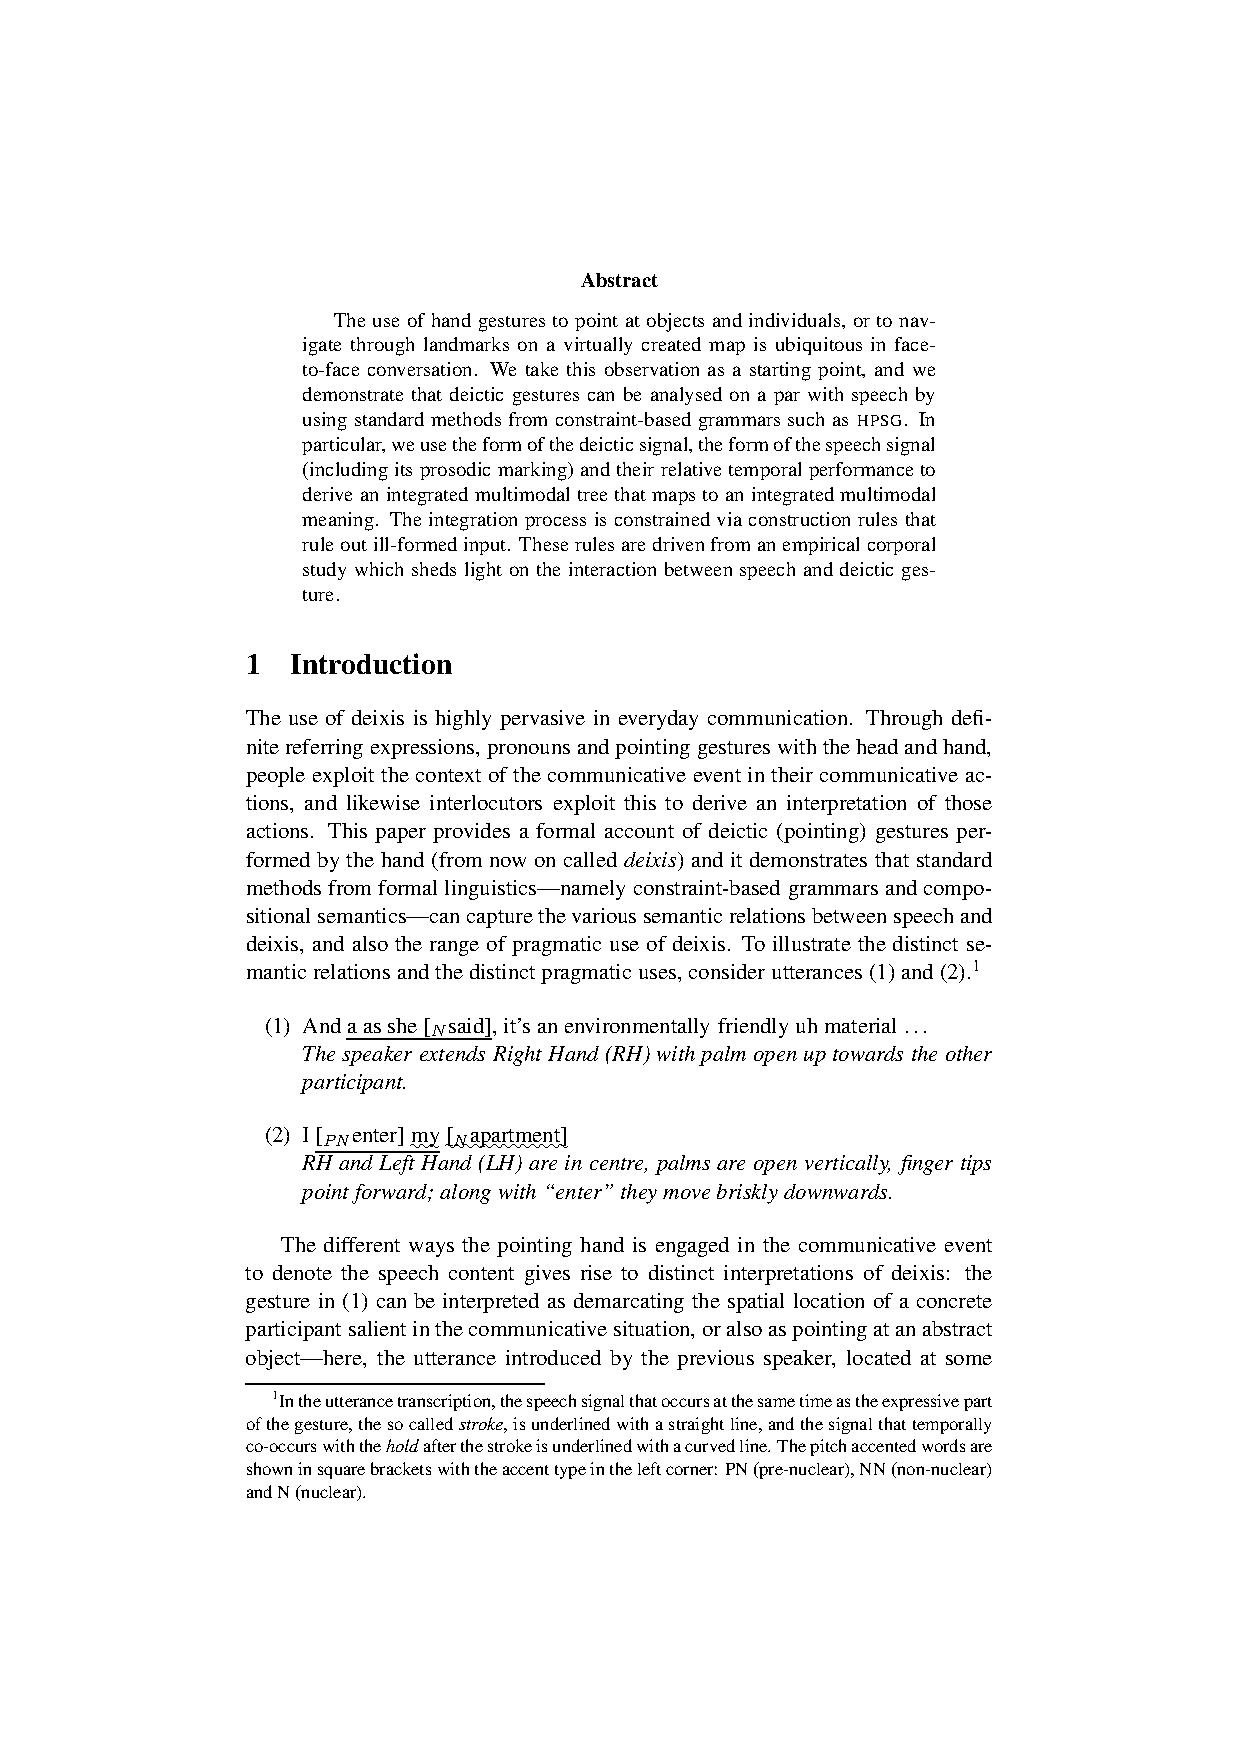
\includepdf[pages=-,pagecommand=\thispagestyle{plain}]{Includes/alahverdzhieva-lascarides.pdf}
        \setcounter{page}{25}
        \phantomsection
        \addcontentsline{toc}{section}{Douglas Ball: Morphology in the `Wrong' Place: The Curious Case of Coast Tsimshian Connectives}
\thispagestyle{empty}

\begin{center}
  {\huge\bfseries Morphology in the `Wrong' Place: The Curious Case of Coast Tsimshian Connectives\par}

  \bigskip

~\\
\begingroup
\setlength{\leftskip}{0pt plus 1fill}
\setlength{\rightskip}{0pt plus 1fill}
\setlength{\parindent}{0pt}
\setlength{\parfillskip}{0pt}
  \formatauthor{Douglas Ball}{\begin{tabular}{@{}c@{}}Truman State University\end{tabular}}

\par\endgroup

  \vspace*{8ex}

  Proceedings of the 18th International Conference on\par Head-Driven Phrase Structure Grammar

  \bigskip

  University of Washington

  \medskip

  Stefan Müller (Editor)

  \medskip

  2011

  \medskip

  CSLI Publications

  \medskip

  pages 25--45

  \medskip

  \url{http://csli-publications.stanford.edu/HPSG/2011}
\end{center}
\vfill

\noindent



\vfill
\noindent
% APA Style
Ball, Douglas. 2011. Morphology in the `Wrong' Place: The Curious Case of Coast Tsimshian Connectives. In Müller, Stefan (Ed.), \emph{{Proceedings of the 18th International Conference on Head-Driven Phrase Structure Grammar, University of Washington}}, 25--45. Stanford,
CA: CSLI Publications. \hfill\href{http://creativecommons.org/licenses/by/4.0/}{\includegraphics[height=.75em]{Includes/ccby.eps}}

\newpage
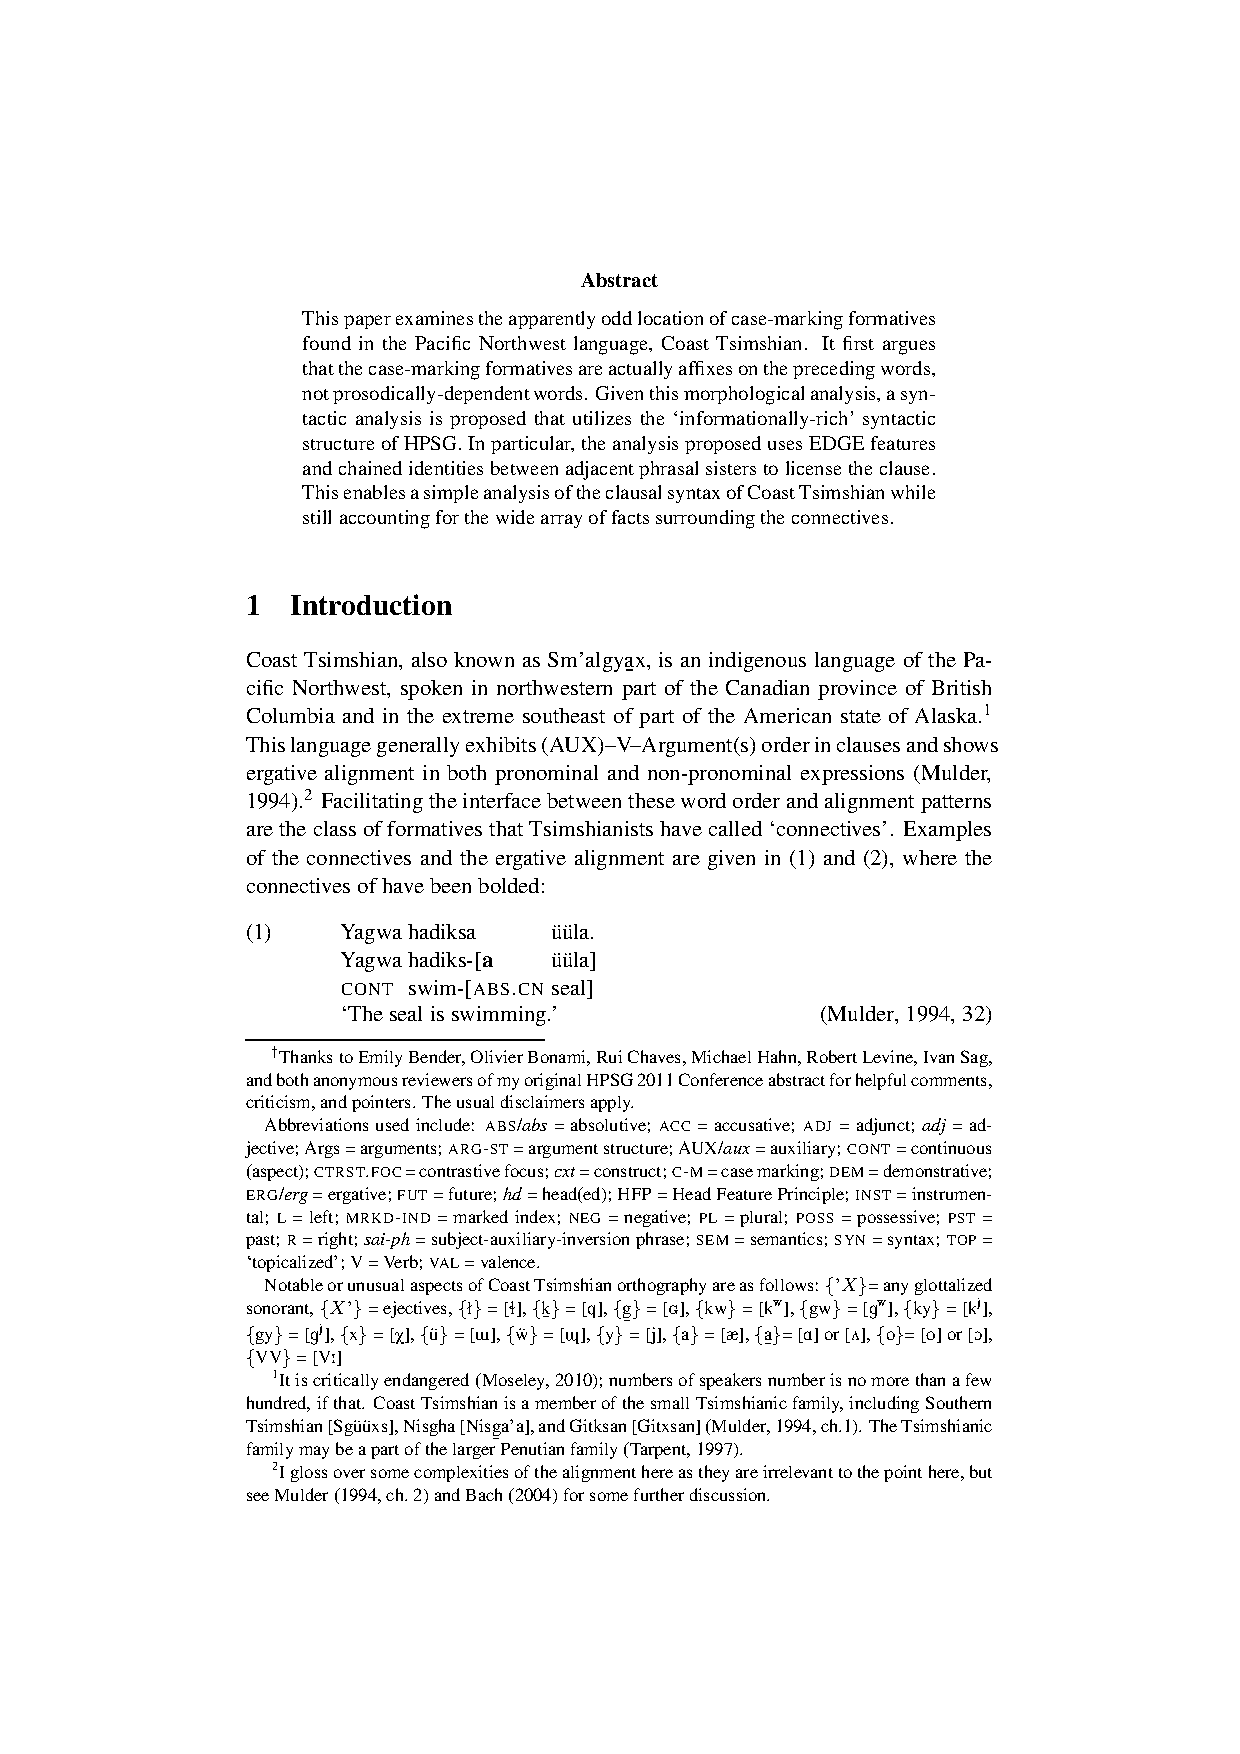
\includepdf[pages=-,pagecommand=\thispagestyle{plain}]{Includes/ball.pdf}
        \setcounter{page}{46}
        \phantomsection
        \addcontentsline{toc}{section}{Joshua Crowgey, Emily M. Bender: Analyzing Interacting Phenomena: Word Order and Negation in Basque}
\thispagestyle{empty}

\begin{center}
  {\huge\bfseries Analyzing Interacting Phenomena: Word Order and Negation in Basque\par}

  \bigskip

~\\
\begingroup
\setlength{\leftskip}{0pt plus 1fill}
\setlength{\rightskip}{0pt plus 1fill}
\setlength{\parindent}{0pt}
\setlength{\parfillskip}{0pt}
  \formatauthor{Joshua Crowgey}{\begin{tabular}{@{}c@{}}University of Washington\end{tabular}}
\formatauthor{Emily M. Bender}{\begin{tabular}{@{}c@{}}University of Washington\end{tabular}}

\par\endgroup

  \vspace*{8ex}

  Proceedings of the 18th International Conference on\par Head-Driven Phrase Structure Grammar

  \bigskip

  University of Washington

  \medskip

  Stefan Müller (Editor)

  \medskip

  2011

  \medskip

  CSLI Publications

  \medskip

  pages 46--59

  \medskip

  \url{http://csli-publications.stanford.edu/HPSG/2011}
\end{center}
\vfill

\noindent



\vfill
\noindent
% APA Style
Crowgey, Joshua, \& Bender, Emily M. 2011. Analyzing Interacting Phenomena: Word Order and Negation in Basque. In Müller, Stefan (Ed.), \emph{{Proceedings of the 18th International Conference on Head-Driven Phrase Structure Grammar, University of Washington}}, 46--59. Stanford,
CA: CSLI Publications. \hfill\href{http://creativecommons.org/licenses/by/4.0/}{\includegraphics[height=.75em]{Includes/ccby.eps}}

\newpage
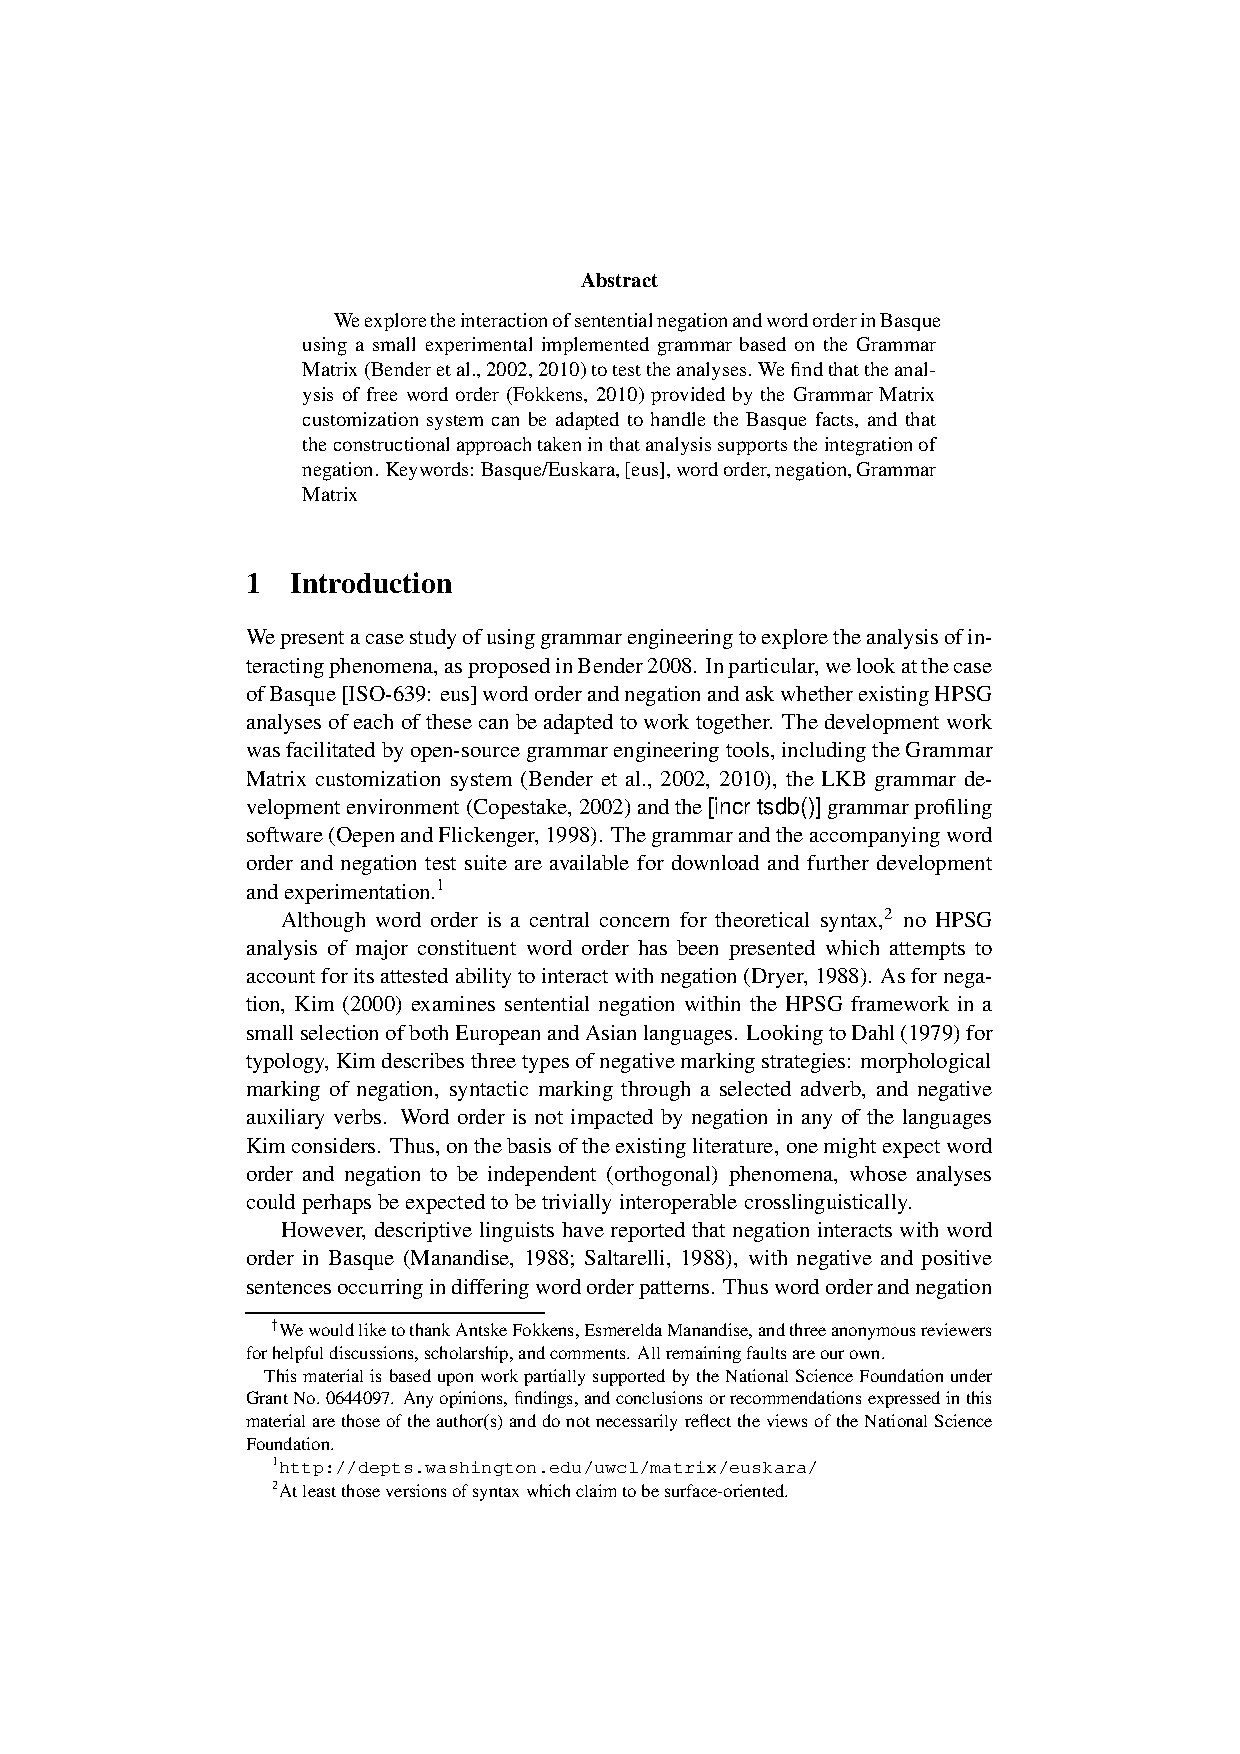
\includepdf[pages=-,pagecommand=\thispagestyle{plain}]{Includes/crowgey-bender.pdf}
        \setcounter{page}{60}
        \phantomsection
        \addcontentsline{toc}{section}{Michael Hahn: Null Conjuncts and Bound Pronouns in Arabic}
\thispagestyle{empty}

\begin{center}
  {\huge\bfseries Null Conjuncts and Bound Pronouns in Arabic\par}

  \bigskip

~\\
\begingroup
\setlength{\leftskip}{0pt plus 1fill}
\setlength{\rightskip}{0pt plus 1fill}
\setlength{\parindent}{0pt}
\setlength{\parfillskip}{0pt}
  \formatauthor{Michael Hahn}{\begin{tabular}{@{}c@{}}University of Tübingen\end{tabular}}

\par\endgroup

  \vspace*{8ex}

  Proceedings of the 18th International Conference on\par Head-Driven Phrase Structure Grammar

  \bigskip

  University of Washington

  \medskip

  Stefan Müller (Editor)

  \medskip

  2011

  \medskip

  CSLI Publications

  \medskip

  pages 60--80

  \medskip

  \url{http://csli-publications.stanford.edu/HPSG/2011}
\end{center}
\vfill

\noindent



\vfill
\noindent
% APA Style
Hahn, Michael. 2011. Null Conjuncts and Bound Pronouns in Arabic. In Müller, Stefan (Ed.), \emph{{Proceedings of the 18th International Conference on Head-Driven Phrase Structure Grammar, University of Washington}}, 60--80. Stanford,
CA: CSLI Publications. \hfill\href{http://creativecommons.org/licenses/by/4.0/}{\includegraphics[height=.75em]{Includes/ccby.eps}}

\newpage
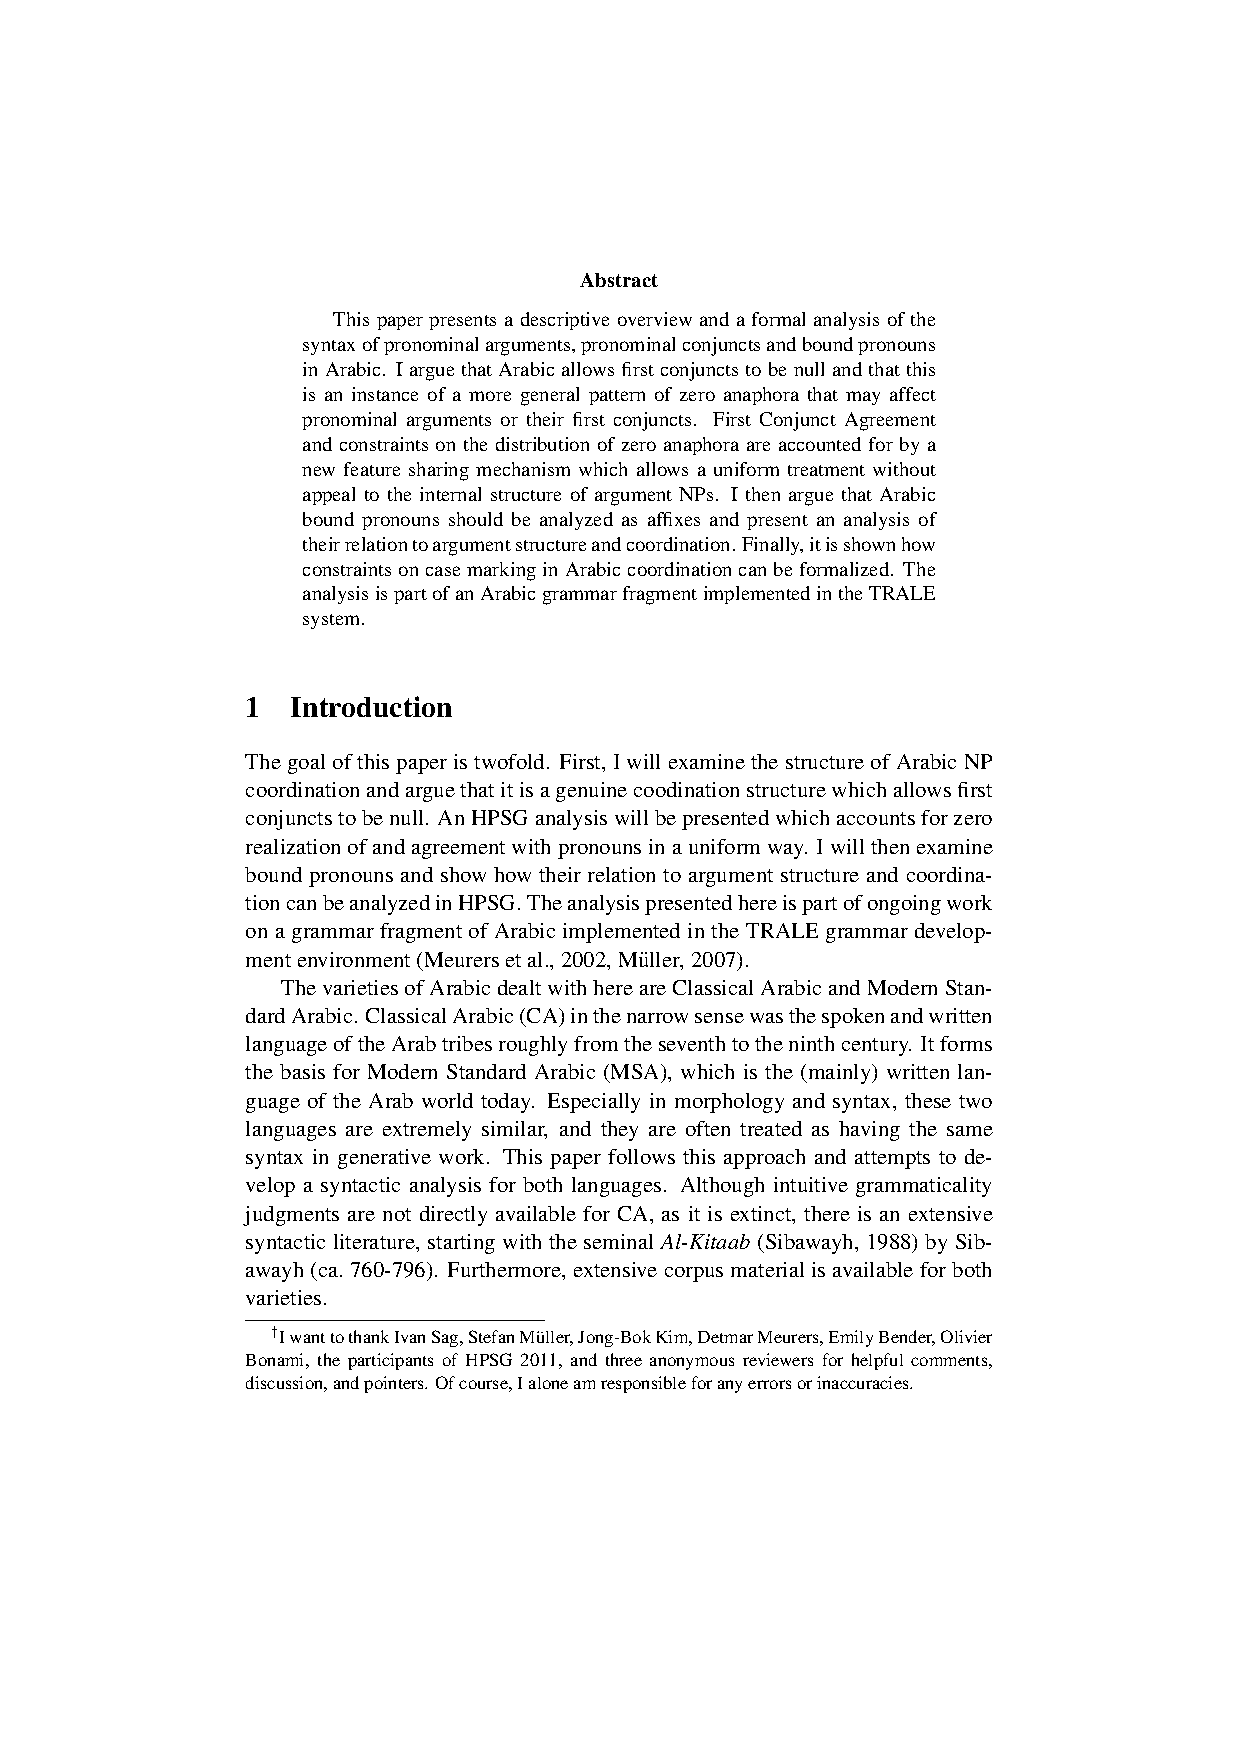
\includepdf[pages=-,pagecommand=\thispagestyle{plain}]{Includes/hahn.pdf}
        \setcounter{page}{81}
        \phantomsection
        \addcontentsline{toc}{section}{Akio Hasegawa, Jean-Pierre Koenig: Focus particles, secondary meanings, and Lexical Resource Semantics:\\ The case of Japanese \emph{shika}}
\thispagestyle{empty}

\begin{center}
  {\huge\bfseries Focus particles, secondary meanings, and Lexical Resource Semantics:\par The case of Japanese \emph{shika}\par}

  \bigskip

~\\
\begingroup
\setlength{\leftskip}{0pt plus 1fill}
\setlength{\rightskip}{0pt plus 1fill}
\setlength{\parindent}{0pt}
\setlength{\parfillskip}{0pt}
  \formatauthor{Akio Hasegawa}{\begin{tabular}{@{}c@{}}University at Buffalo\end{tabular}}
\formatauthor{Jean-Pierre Koenig}{\begin{tabular}{@{}c@{}}University at Buffalo\end{tabular}}

\par\endgroup

  \vspace*{8ex}

  Proceedings of the 18th International Conference on\par Head-Driven Phrase Structure Grammar

  \bigskip

  University of Washington

  \medskip

  Stefan Müller (Editor)

  \medskip

  2011

  \medskip

  CSLI Publications

  \medskip

  pages 81--101

  \medskip

  \url{http://csli-publications.stanford.edu/HPSG/2011}
\end{center}
\vfill

\noindent



\vfill
\noindent
% APA Style
Hasegawa, Akio, \& Koenig,  Jean-Pierre. 2011. Focus particles, secondary meanings, and Lexical Resource Semantics:  The case of Japanese \emph{shika}. In Müller, Stefan (Ed.), \emph{{Proceedings of the 18th International Conference on Head-Driven Phrase Structure Grammar, University of Washington}}, 81--101. Stanford,
CA: CSLI Publications. \hfill\href{http://creativecommons.org/licenses/by/4.0/}{\includegraphics[height=.75em]{Includes/ccby.eps}}

\newpage
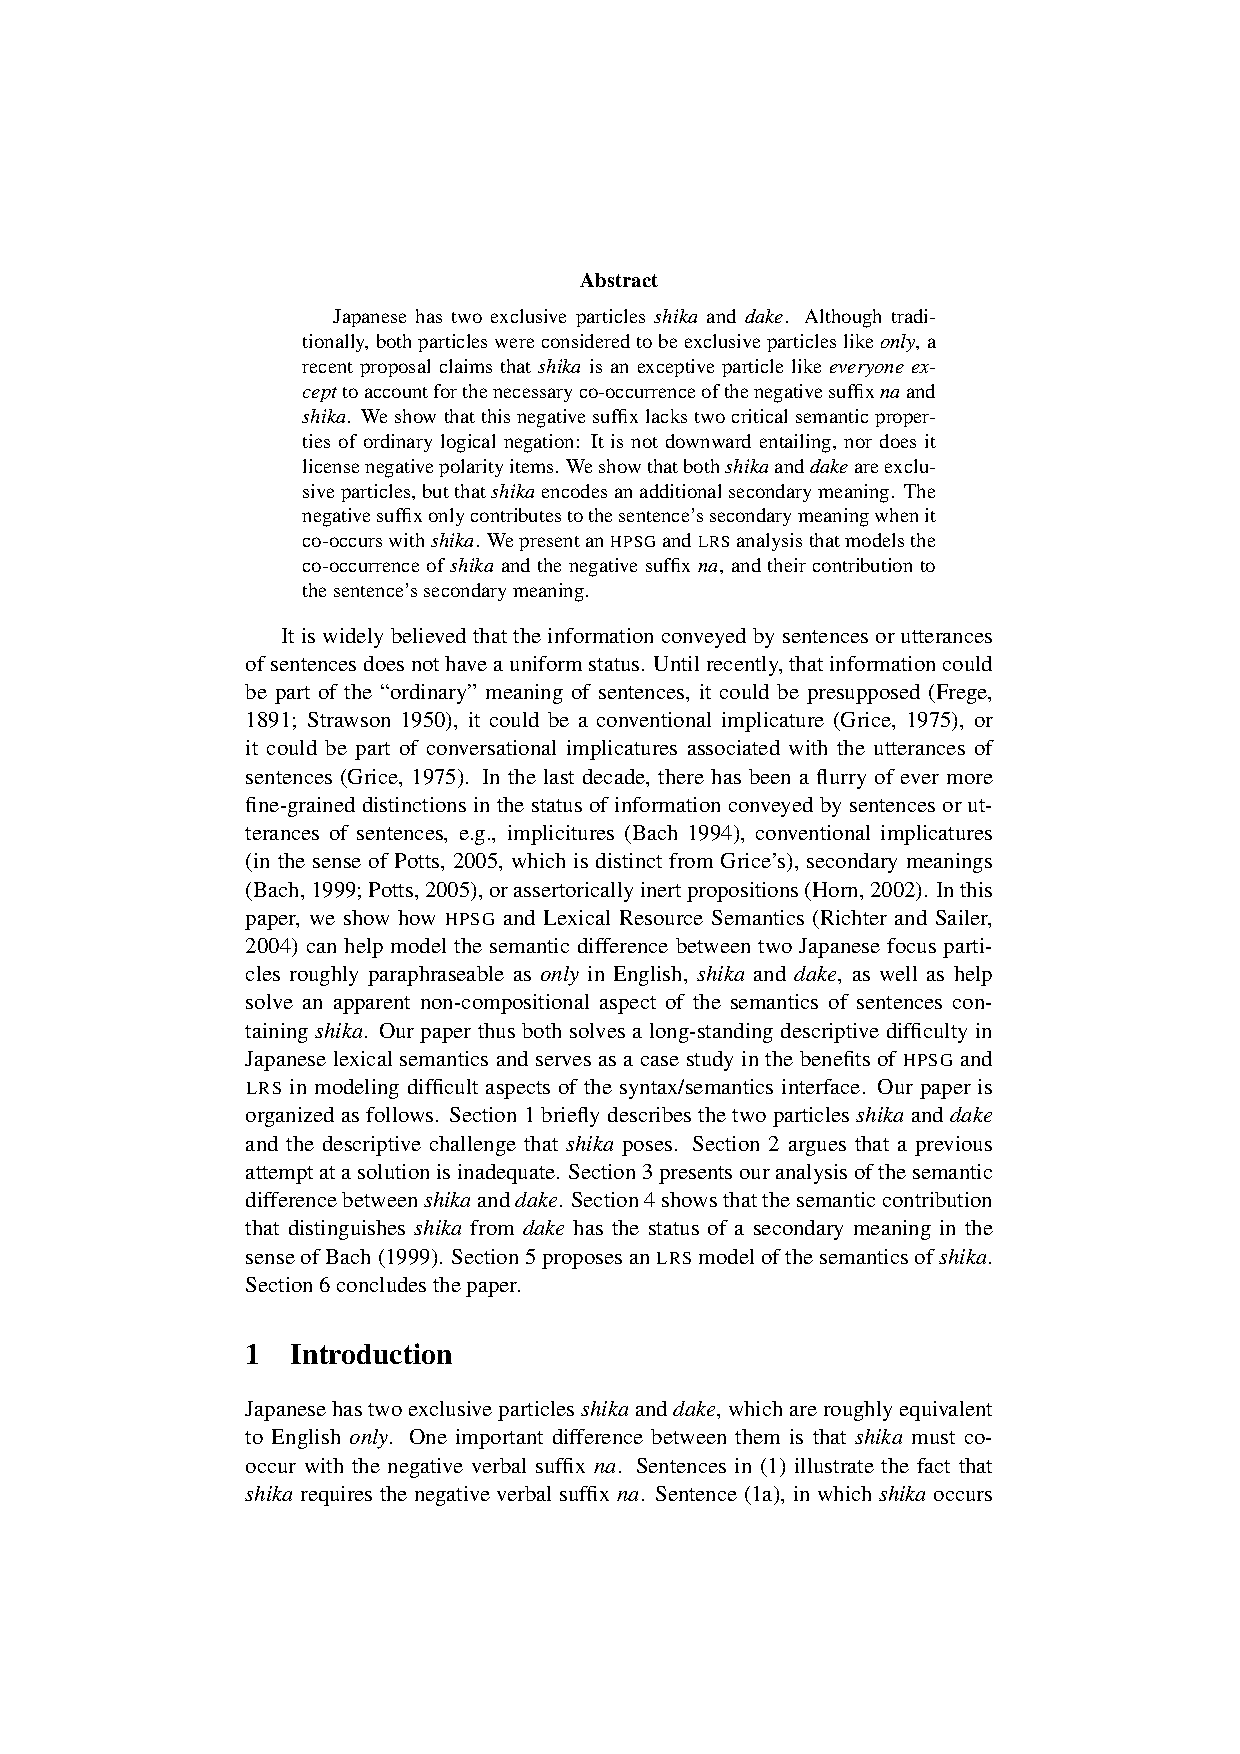
\includepdf[pages=-,pagecommand=\thispagestyle{plain}]{Includes/hasegawa-koenig.pdf}
        \setcounter{page}{102}
        \phantomsection
        \addcontentsline{toc}{section}{Jong-Bok Kim, Peter Sells: The English Binominal NP Construction: A Construction-Based Perspective}
\thispagestyle{empty}

\begin{center}
  {\huge\bfseries The English Binominal NP Construction: A Construction-Based Perspective\par}

  \bigskip

~\\
\begingroup
\setlength{\leftskip}{0pt plus 1fill}
\setlength{\rightskip}{0pt plus 1fill}
\setlength{\parindent}{0pt}
\setlength{\parfillskip}{0pt}
  \formatauthor{Jong-Bok Kim}{\begin{tabular}{@{}c@{}}Kyung Hee University\end{tabular}}
\formatauthor{Peter Sells}{\begin{tabular}{@{}c@{}}University of York\end{tabular}}

\par\endgroup

  \vspace*{8ex}

  Proceedings of the 18th International Conference on\par Head-Driven Phrase Structure Grammar

  \bigskip

  University of Washington

  \medskip

  Stefan Müller (Editor)

  \medskip

  2011

  \medskip

  CSLI Publications

  \medskip

  pages 102--108

  \medskip

  \url{http://csli-publications.stanford.edu/HPSG/2011}
\end{center}
\vfill

\noindent



\vfill
\noindent
% APA Style
Kim, Jong-Bok, \& Sells, Peter. 2011. The English Binominal NP Construction: A Construction-Based Perspective. In Müller, Stefan (Ed.), \emph{{Proceedings of the 18th International Conference on Head-Driven Phrase Structure Grammar, University of Washington}}, 102--108. Stanford,
CA: CSLI Publications. \hfill\href{http://creativecommons.org/licenses/by/4.0/}{\includegraphics[height=.75em]{Includes/ccby.eps}}

\newpage
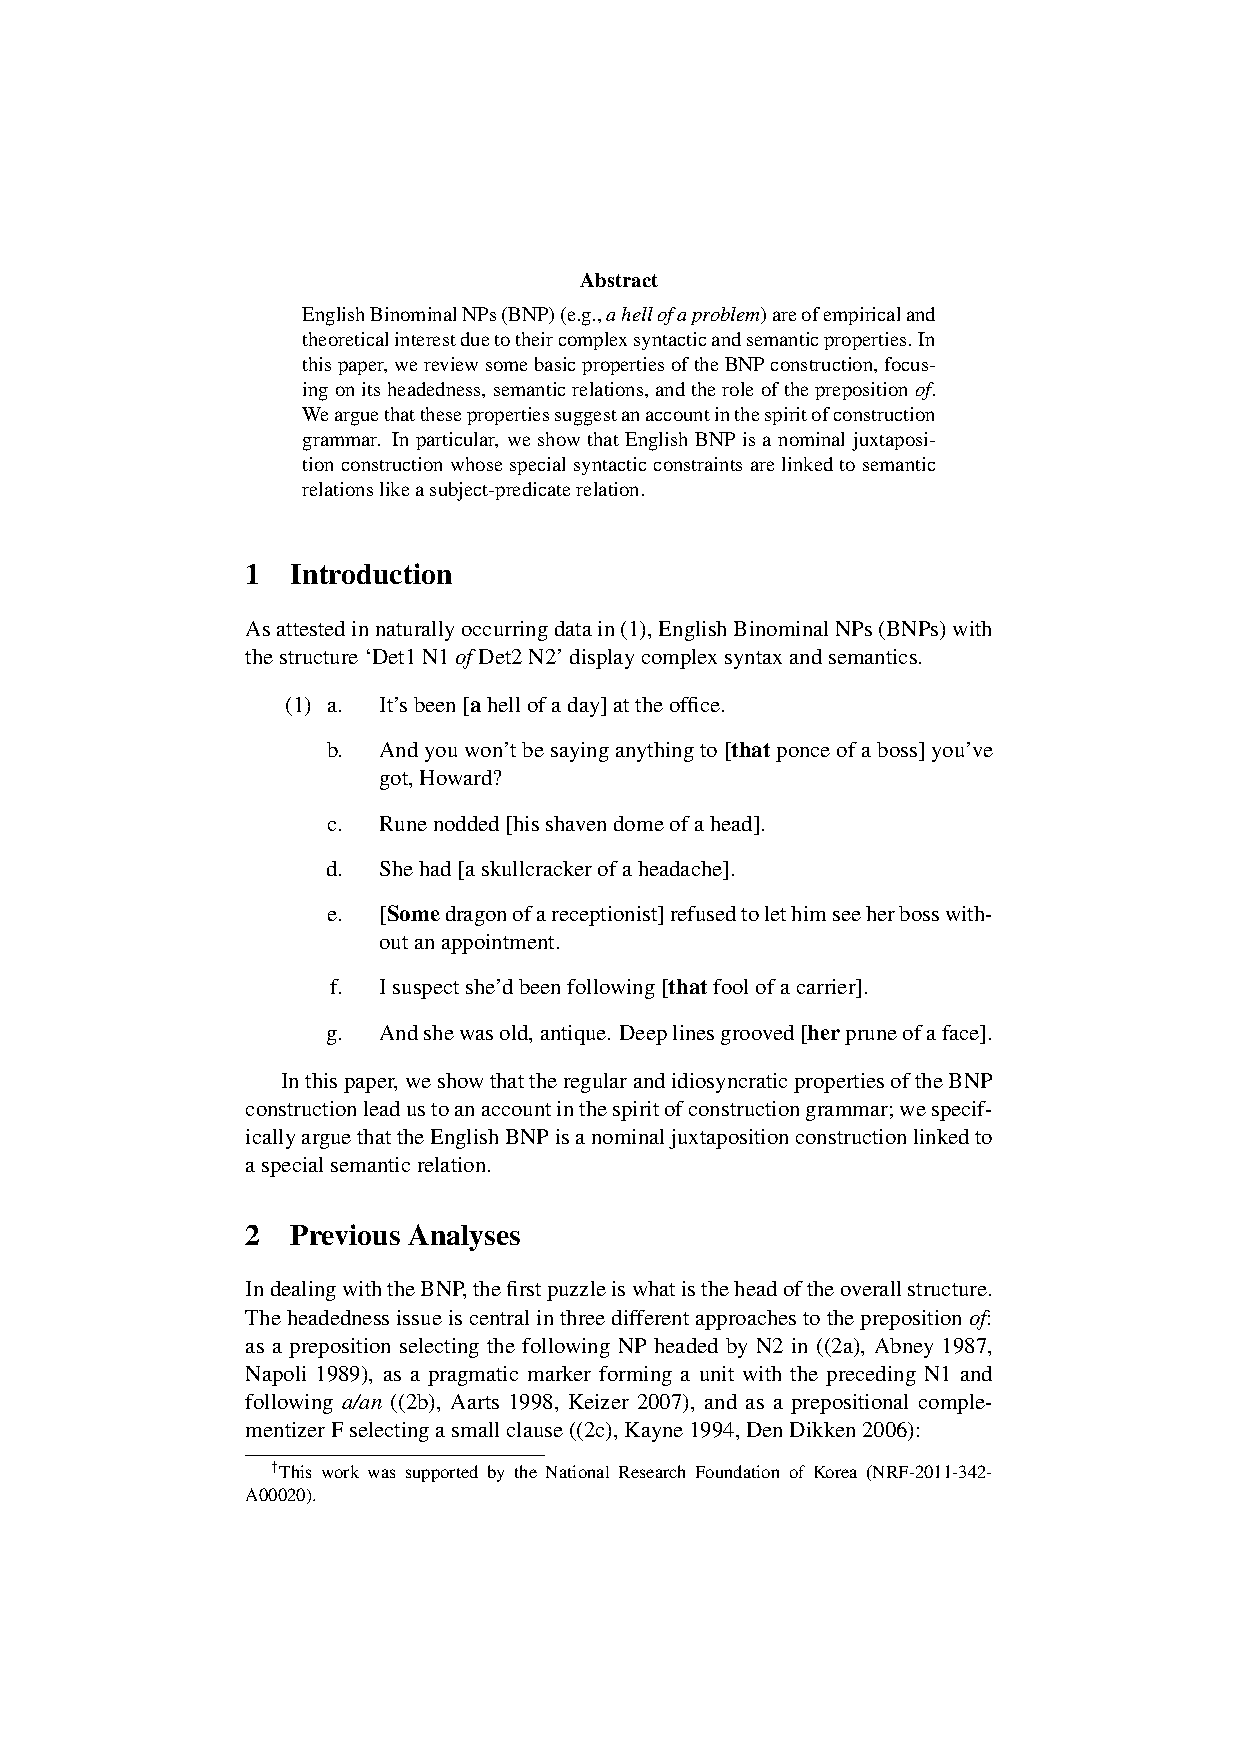
\includepdf[pages=-,pagecommand=\thispagestyle{plain}]{Includes/kim-sells.pdf}
        \setcounter{page}{109}
        \phantomsection
        \addcontentsline{toc}{section}{Hans-Ulrich Krieger, Bernd Kiefer: Converting CCGs into Typed Feature Structure Grammars}
\thispagestyle{empty}

\begin{center}
  {\huge\bfseries Converting CCGs into Typed Feature Structure Grammars\par}

  \bigskip

~\\
\begingroup
\setlength{\leftskip}{0pt plus 1fill}
\setlength{\rightskip}{0pt plus 1fill}
\setlength{\parindent}{0pt}
\setlength{\parfillskip}{0pt}
  \formatauthor{Hans-Ulrich Krieger}{\begin{tabular}{@{}c@{}}DFKI, Saarbrücken\end{tabular}}
\formatauthor{Bernd Kiefer}{\begin{tabular}{@{}c@{}}DFKI, Saarbrücken\end{tabular}}

\par\endgroup

  \vspace*{8ex}

  Proceedings of the 18th International Conference on\par Head-Driven Phrase Structure Grammar

  \bigskip

  University of Washington

  \medskip

  Stefan Müller (Editor)

  \medskip

  2011

  \medskip

  CSLI Publications

  \medskip

  pages 109--125

  \medskip

  \url{http://csli-publications.stanford.edu/HPSG/2011}
\end{center}
\vfill

\noindent



\vfill
\noindent
% APA Style
Krieger, Hans-Ulrich, \& Kiefer, Bernd. 2011. Converting CCGs into Typed Feature Structure Grammars. In Müller, Stefan (Ed.), \emph{{Proceedings of the 18th International Conference on Head-Driven Phrase Structure Grammar, University of Washington}}, 109--125. Stanford,
CA: CSLI Publications. \hfill\href{http://creativecommons.org/licenses/by/4.0/}{\includegraphics[height=.75em]{Includes/ccby.eps}}

\newpage
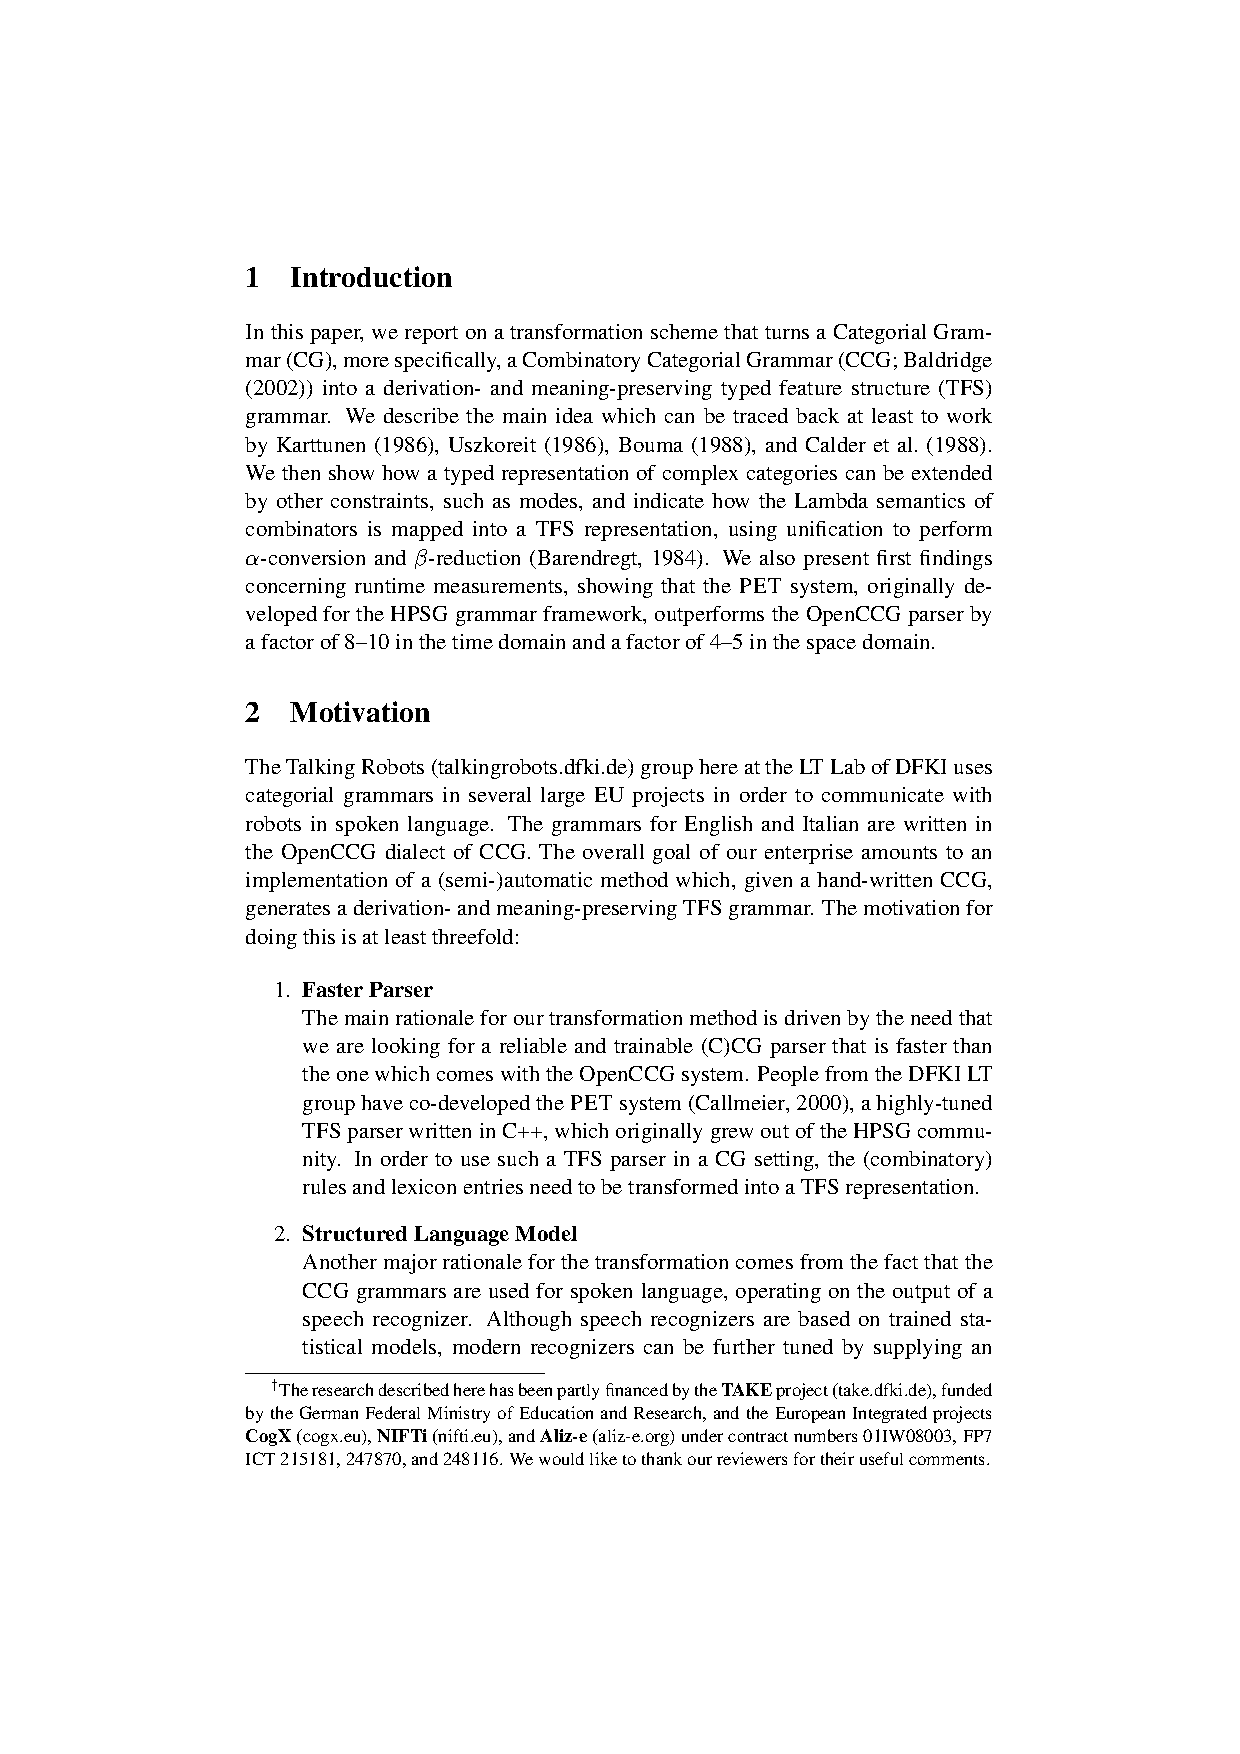
\includepdf[pages=-,pagecommand=\thispagestyle{plain}]{Includes/krieger-kiefer.pdf}
        \setcounter{page}{126}
        \phantomsection
        \addcontentsline{toc}{section}{Robert Levine: Linearization and its discontents}
\thispagestyle{empty}

\begin{center}
  {\huge\bfseries Linearization and its discontents\par}

  \bigskip

~\\
\begingroup
\setlength{\leftskip}{0pt plus 1fill}
\setlength{\rightskip}{0pt plus 1fill}
\setlength{\parindent}{0pt}
\setlength{\parfillskip}{0pt}
  \formatauthor{Robert Levine}{\begin{tabular}{@{}c@{}}Ohio State University\end{tabular}}

\par\endgroup

  \vspace*{8ex}

  Proceedings of the 18th International Conference on\par Head-Driven Phrase Structure Grammar

  \bigskip

  University of Washington

  \medskip

  Stefan Müller (Editor)

  \medskip

  2011

  \medskip

  CSLI Publications

  \medskip

  pages 126--146

  \medskip

  \url{http://csli-publications.stanford.edu/HPSG/2011}
\end{center}
\vfill

\noindent



\vfill
\noindent
% APA Style
Levine, Robert. 2011. Linearization and its discontents. In Müller, Stefan (Ed.), \emph{{Proceedings of the 18th International Conference on Head-Driven Phrase Structure Grammar, University of Washington}}, 126--146. Stanford,
CA: CSLI Publications. \hfill\href{http://creativecommons.org/licenses/by/4.0/}{\includegraphics[height=.75em]{Includes/ccby.eps}}

\newpage
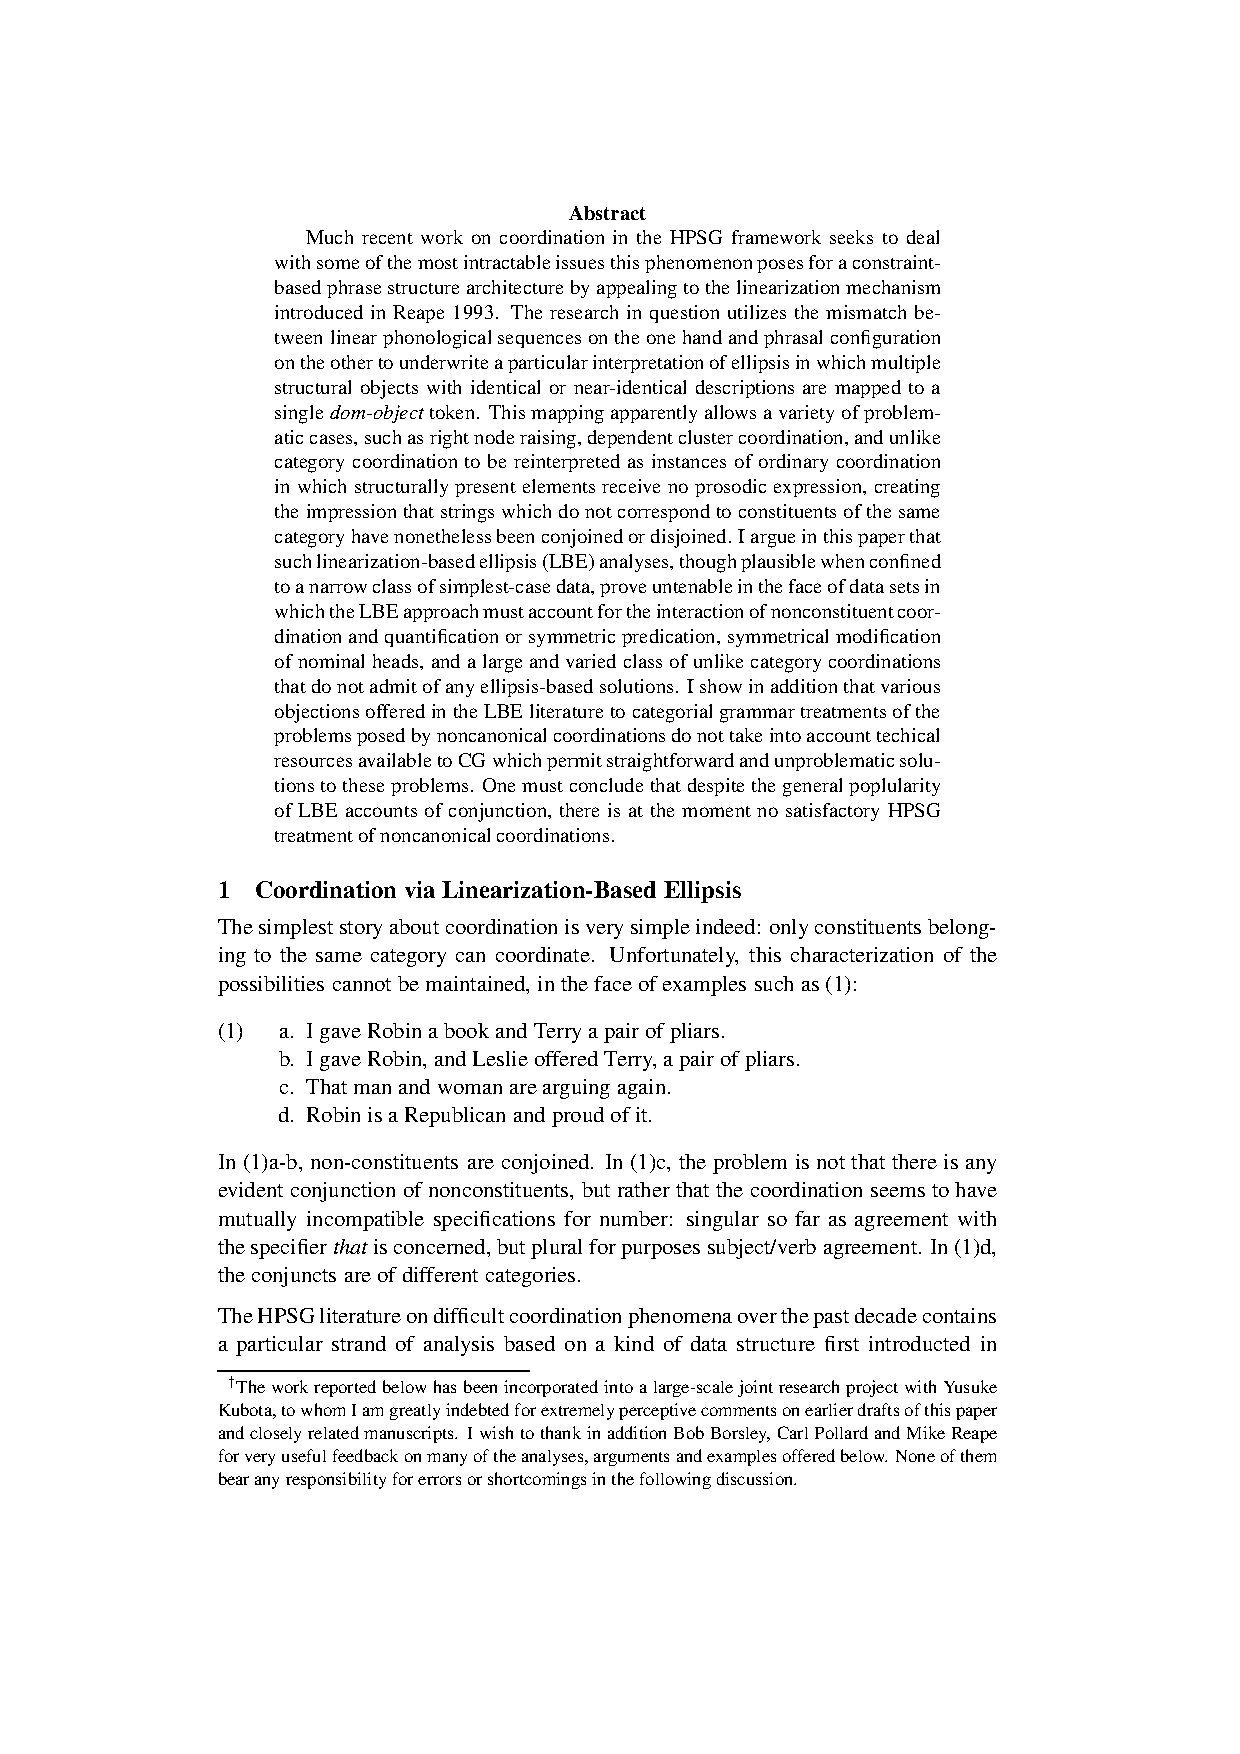
\includepdf[pages=-,pagecommand=\thispagestyle{plain}]{Includes/levine.pdf}
        \setcounter{page}{147}
        \phantomsection
        \addcontentsline{toc}{section}{Janna Lipenkova: Reanalysis of semantically required dependents as complements in the Chinese \emph{ba}-construction}
\thispagestyle{empty}

\begin{center}
  {\huge\bfseries Reanalysis of semantically required dependents as complements in the Chinese \emph{ba}-construction\par}

  \bigskip

~\\
\begingroup
\setlength{\leftskip}{0pt plus 1fill}
\setlength{\rightskip}{0pt plus 1fill}
\setlength{\parindent}{0pt}
\setlength{\parfillskip}{0pt}
  \formatauthor{Janna Lipenkova}{\begin{tabular}{@{}c@{}}Freie Universität Berlin\end{tabular}}

\par\endgroup

  \vspace*{8ex}

  Proceedings of the 18th International Conference on\par Head-Driven Phrase Structure Grammar

  \bigskip

  University of Washington

  \medskip

  Stefan Müller (Editor)

  \medskip

  2011

  \medskip

  CSLI Publications

  \medskip

  pages 147--166

  \medskip

  \url{http://csli-publications.stanford.edu/HPSG/2011}
\end{center}
\vfill

\noindent



\vfill
\noindent
% APA Style
Lipenkova, Janna. 2011. Reanalysis of semantically required dependents as complements in the Chinese \emph{ba}-construction. In Müller, Stefan (Ed.), \emph{{Proceedings of the 18th International Conference on Head-Driven Phrase Structure Grammar, University of Washington}}, 147--166. Stanford,
CA: CSLI Publications. \hfill\href{http://creativecommons.org/licenses/by/4.0/}{\includegraphics[height=.75em]{Includes/ccby.eps}}

\newpage
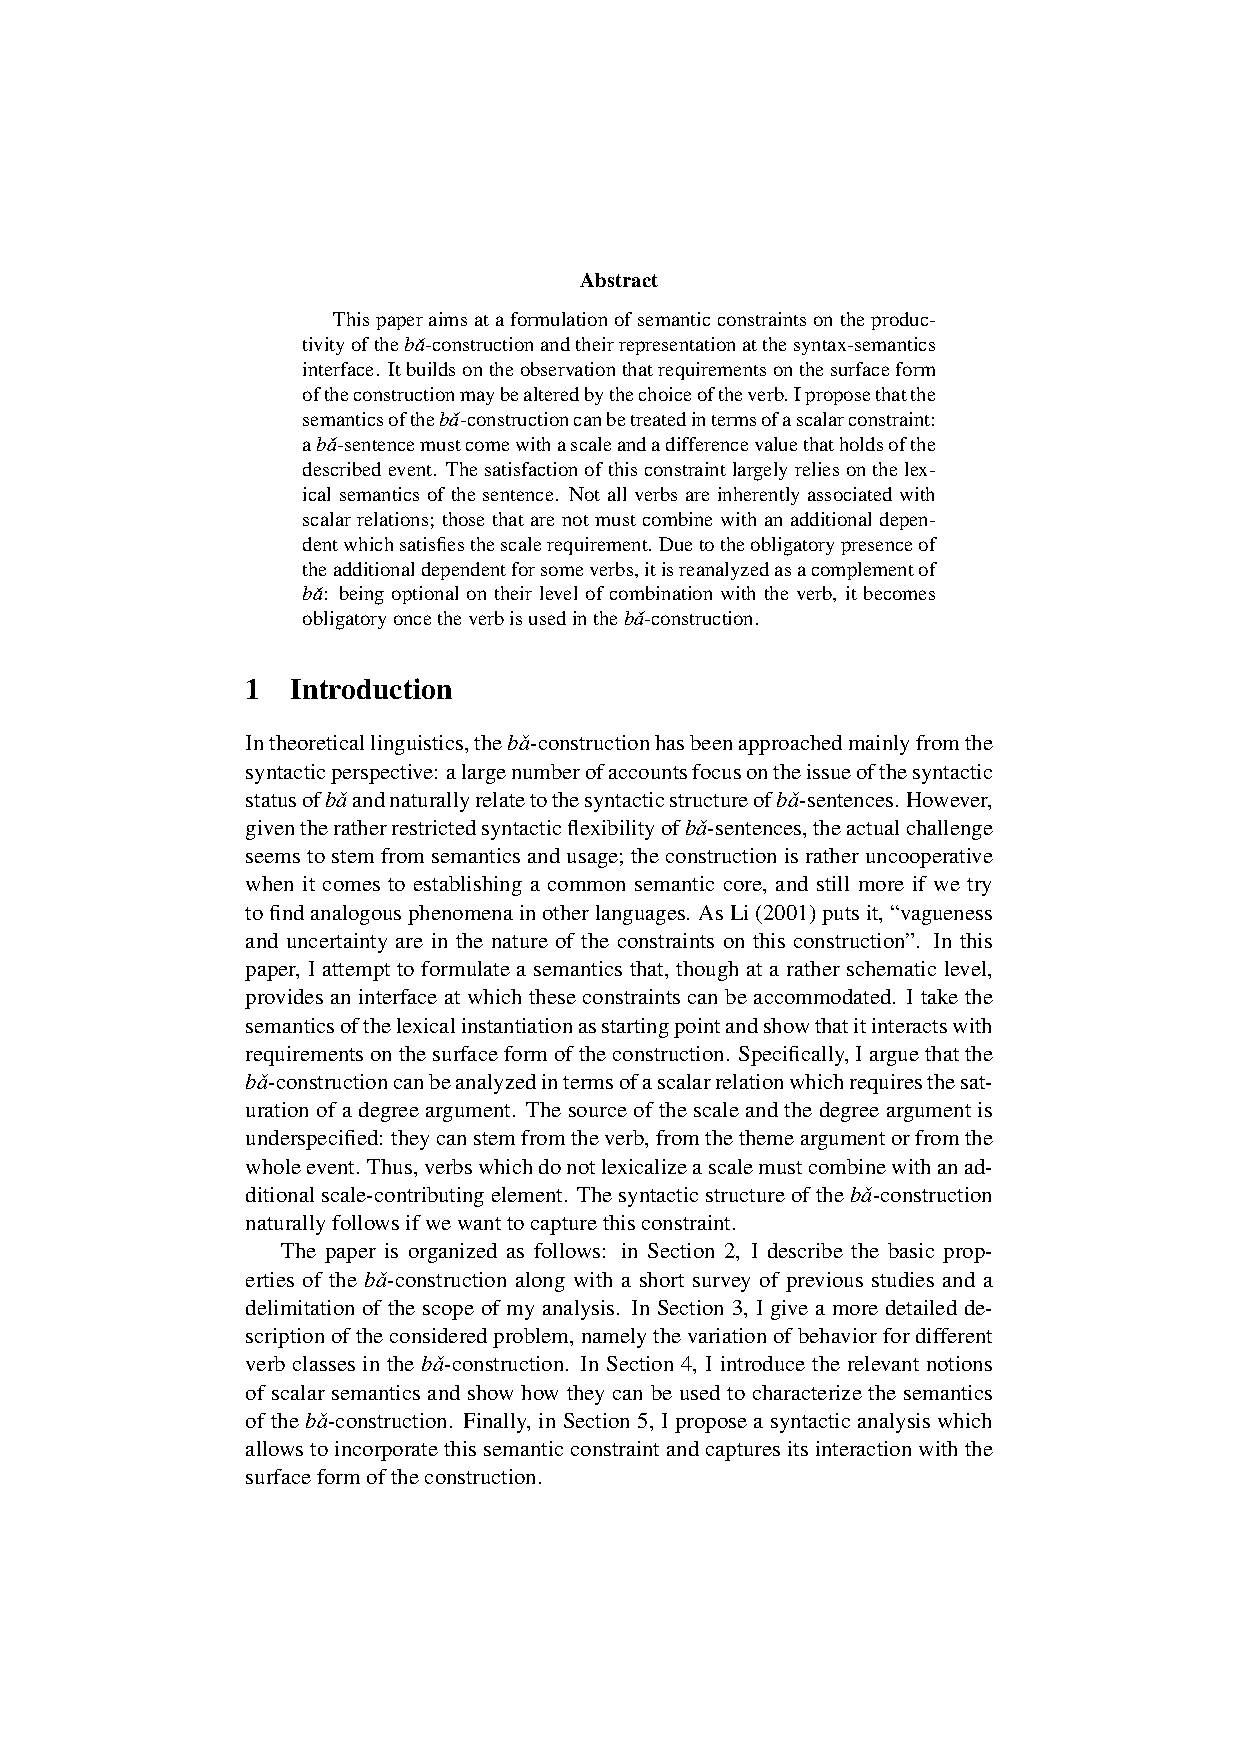
\includepdf[pages=-,pagecommand=\thispagestyle{plain}]{Includes/lipenkova.pdf}
        \setcounter{page}{167}
        \phantomsection
        \addcontentsline{toc}{section}{Stefan M{\"u}ller, Bjarne {\O}rsnes: Positional Expletives in Danish, German, and Yiddish}
\thispagestyle{empty}

\begin{center}
  {\huge\bfseries Positional Expletives in Danish, German, and Yiddish\par}

  \bigskip

~\\
\begingroup
\setlength{\leftskip}{0pt plus 1fill}
\setlength{\rightskip}{0pt plus 1fill}
\setlength{\parindent}{0pt}
\setlength{\parfillskip}{0pt}
  \formatauthor{Stefan Müller}{\begin{tabular}{@{}c@{}}Freie Universität Berlin\end{tabular}}
\formatauthor{Bjarne Ørsnes}{\begin{tabular}{@{}c@{}}Freie Universität Berlin\end{tabular}}

\par\endgroup

  \vspace*{8ex}

  Proceedings of the 18th International Conference on\par Head-Driven Phrase Structure Grammar

  \bigskip

  University of Washington

  \medskip

  Stefan Müller (Editor)

  \medskip

  2011

  \medskip

  CSLI Publications

  \medskip

  pages 167--187

  \medskip

  \url{http://csli-publications.stanford.edu/HPSG/2011}
\end{center}
\vfill

\noindent



\vfill
\noindent
% APA Style
Müller, Stefan, \& Ørsnes,  Bjarne. 2011. Positional Expletives in Danish, German, and Yiddish. In Müller, Stefan (Ed.), \emph{{Proceedings of the 18th International Conference on Head-Driven Phrase Structure Grammar, University of Washington}}, 167--187. Stanford,
CA: CSLI Publications. \hfill\href{http://creativecommons.org/licenses/by/4.0/}{\includegraphics[height=.75em]{Includes/ccby.eps}}

\newpage
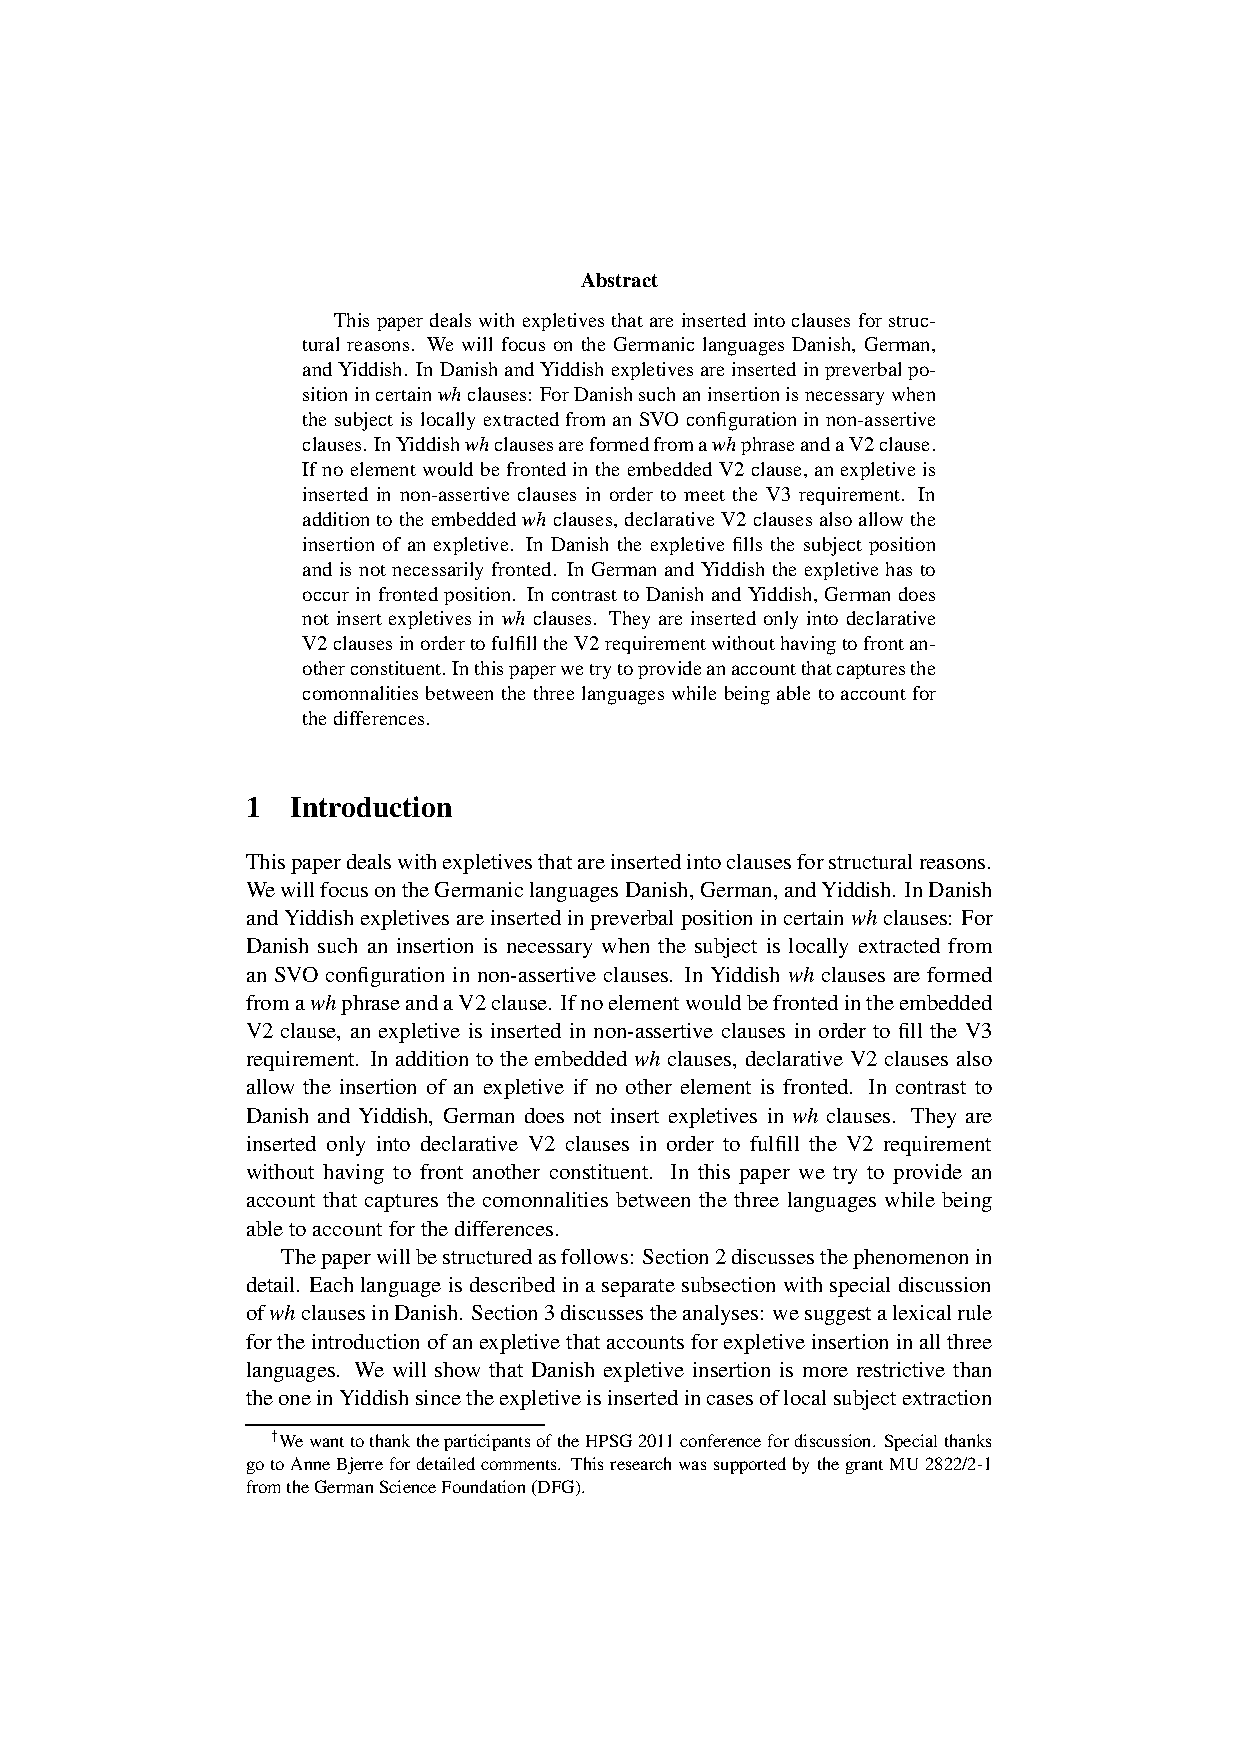
\includepdf[pages=-,pagecommand=\thispagestyle{plain}]{Includes/mueller-oersnes.pdf}
        \setcounter{page}{188}
        \phantomsection
        \addcontentsline{toc}{section}{Ivan A. Sag, Joanna Nykiel: Remarks on Sluicing}
\thispagestyle{empty}

\begin{center}
  {\huge\bfseries Remarks on Sluicing\par}

  \bigskip

~\\
\begingroup
\setlength{\leftskip}{0pt plus 1fill}
\setlength{\rightskip}{0pt plus 1fill}
\setlength{\parindent}{0pt}
\setlength{\parfillskip}{0pt}
  \formatauthor{Ivan A. Sag}{\begin{tabular}{@{}c@{}}Stanford University\end{tabular}}
\formatauthor{Joanna Nykiel}{\begin{tabular}{@{}c@{}}University of Silesia\end{tabular}}

\par\endgroup

  \vspace*{8ex}

  Proceedings of the 18th International Conference on\par Head-Driven Phrase Structure Grammar

  \bigskip

  University of Washington

  \medskip

  Stefan Müller (Editor)

  \medskip

  2011

  \medskip

  CSLI Publications

  \medskip

  pages 188--208

  \medskip

  \url{http://csli-publications.stanford.edu/HPSG/2011}
\end{center}
\vfill

\noindent



\vfill
\noindent
% APA Style
Sag, Ivan A., \& Nykiel, Joanna. 2011. Remarks on Sluicing. In Müller, Stefan (Ed.), \emph{{Proceedings of the 18th International Conference on Head-Driven Phrase Structure Grammar, University of Washington}}, 188--208. Stanford,
CA: CSLI Publications. \hfill\href{http://creativecommons.org/licenses/by/4.0/}{\includegraphics[height=.75em]{Includes/ccby.eps}}

\newpage
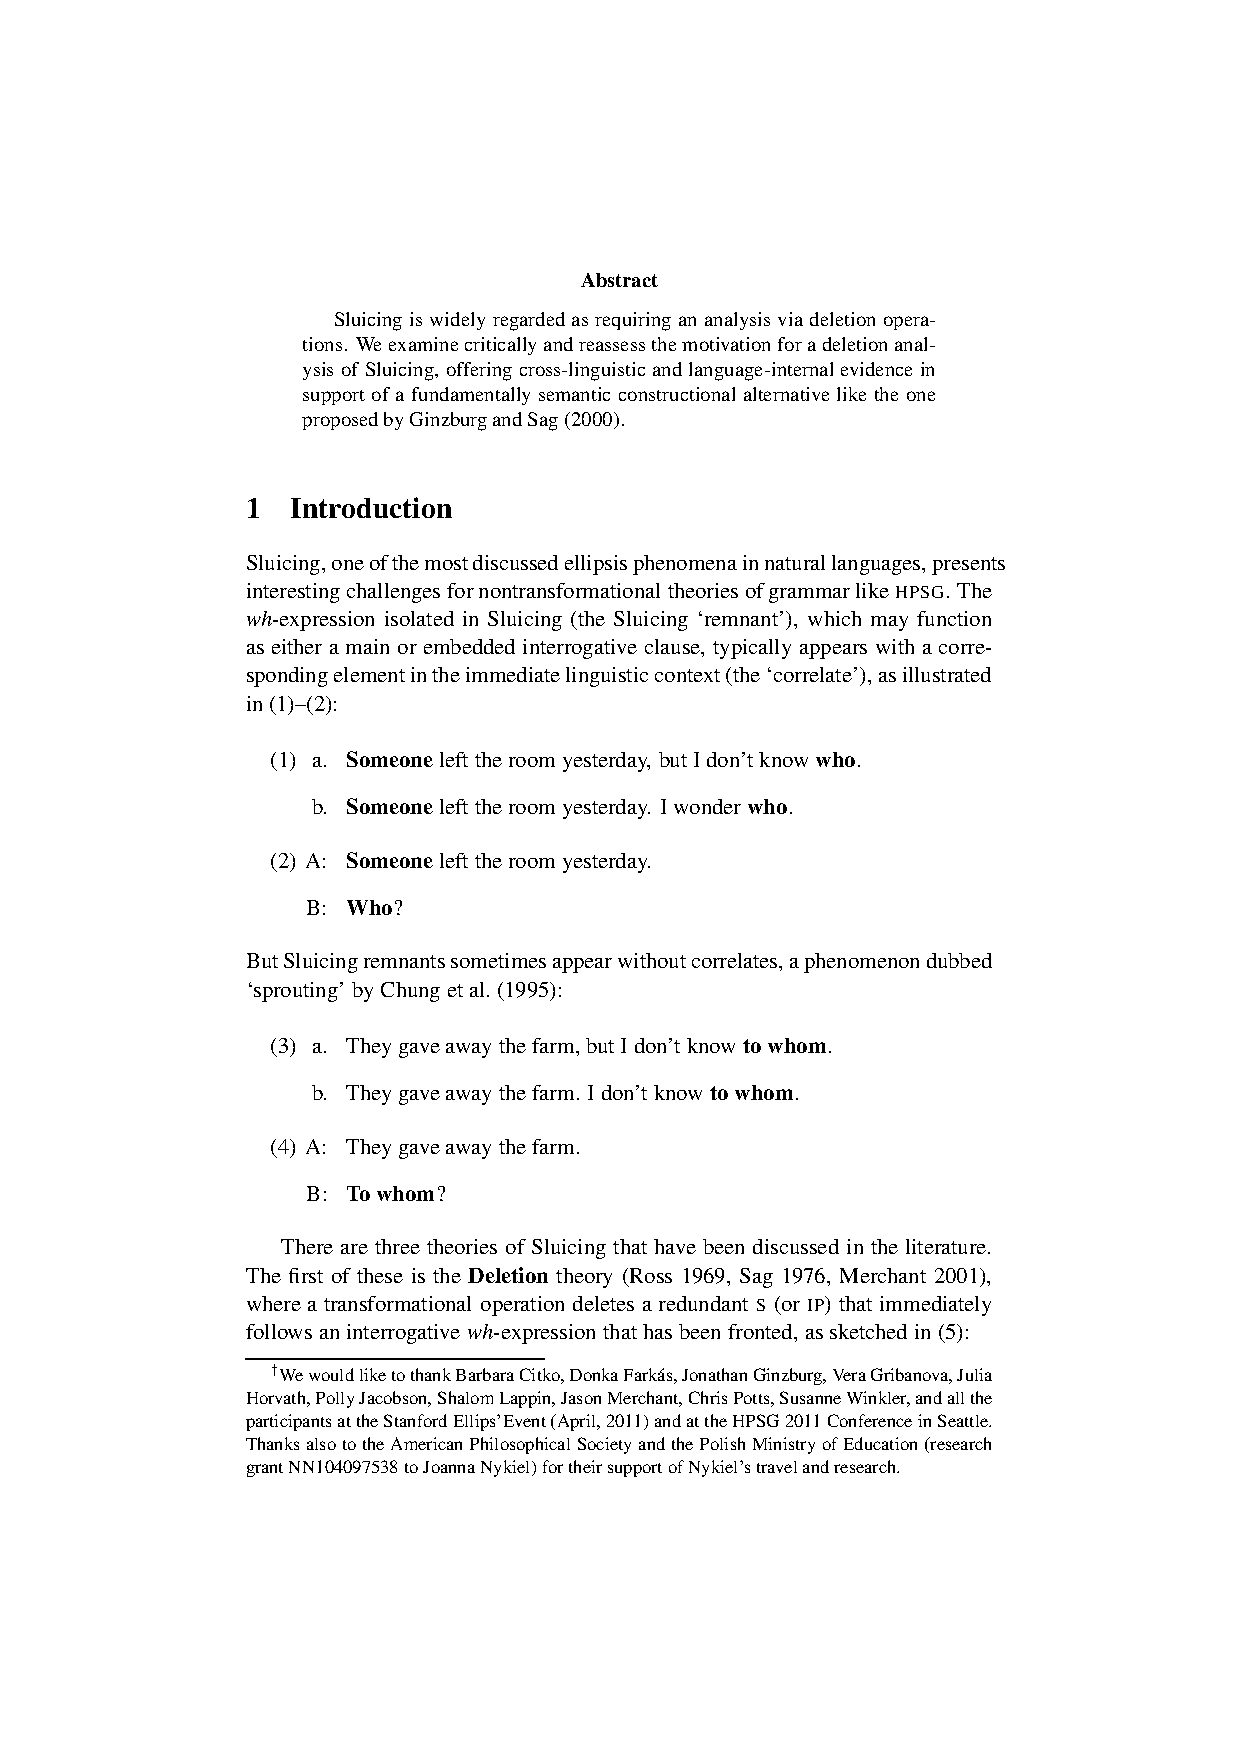
\includepdf[pages=-,pagecommand=\thispagestyle{plain}]{Includes/sag-nykiel.pdf}
        \setcounter{page}{209}
        \phantomsection
        \addcontentsline{toc}{section}{Juliette Thuilier: Case Suffixes and Postpositions in Hungarian}
\thispagestyle{empty}

\begin{center}
  {\huge\bfseries Case Suffixes and Postpositions in Hungarian\par}

  \bigskip

~\\
\begingroup
\setlength{\leftskip}{0pt plus 1fill}
\setlength{\rightskip}{0pt plus 1fill}
\setlength{\parindent}{0pt}
\setlength{\parfillskip}{0pt}
  \formatauthor{Juliette Thuilier}{\begin{tabular}{@{}c@{}}Univ Paris Diderot, Sorbonne Paris Cité, ALPAGE, UMR-I 001 INRIA\end{tabular}}

\par\endgroup

  \vspace*{8ex}

  Proceedings of the 18th International Conference on\par Head-Driven Phrase Structure Grammar

  \bigskip

  University of Washington

  \medskip

  Stefan Müller (Editor)

  \medskip

  2011

  \medskip

  CSLI Publications

  \medskip

  pages 209--226

  \medskip

  \url{http://csli-publications.stanford.edu/HPSG/2011}
\end{center}
\vfill

\noindent



\vfill
\noindent
% APA Style
Thuilier, Juliette. 2011. Case Suffixes and Postpositions in Hungarian. In Müller, Stefan (Ed.), \emph{{Proceedings of the 18th International Conference on Head-Driven Phrase Structure Grammar, University of Washington}}, 209--226. Stanford,
CA: CSLI Publications. \hfill\href{http://creativecommons.org/licenses/by/4.0/}{\includegraphics[height=.75em]{Includes/ccby.eps}}

\newpage
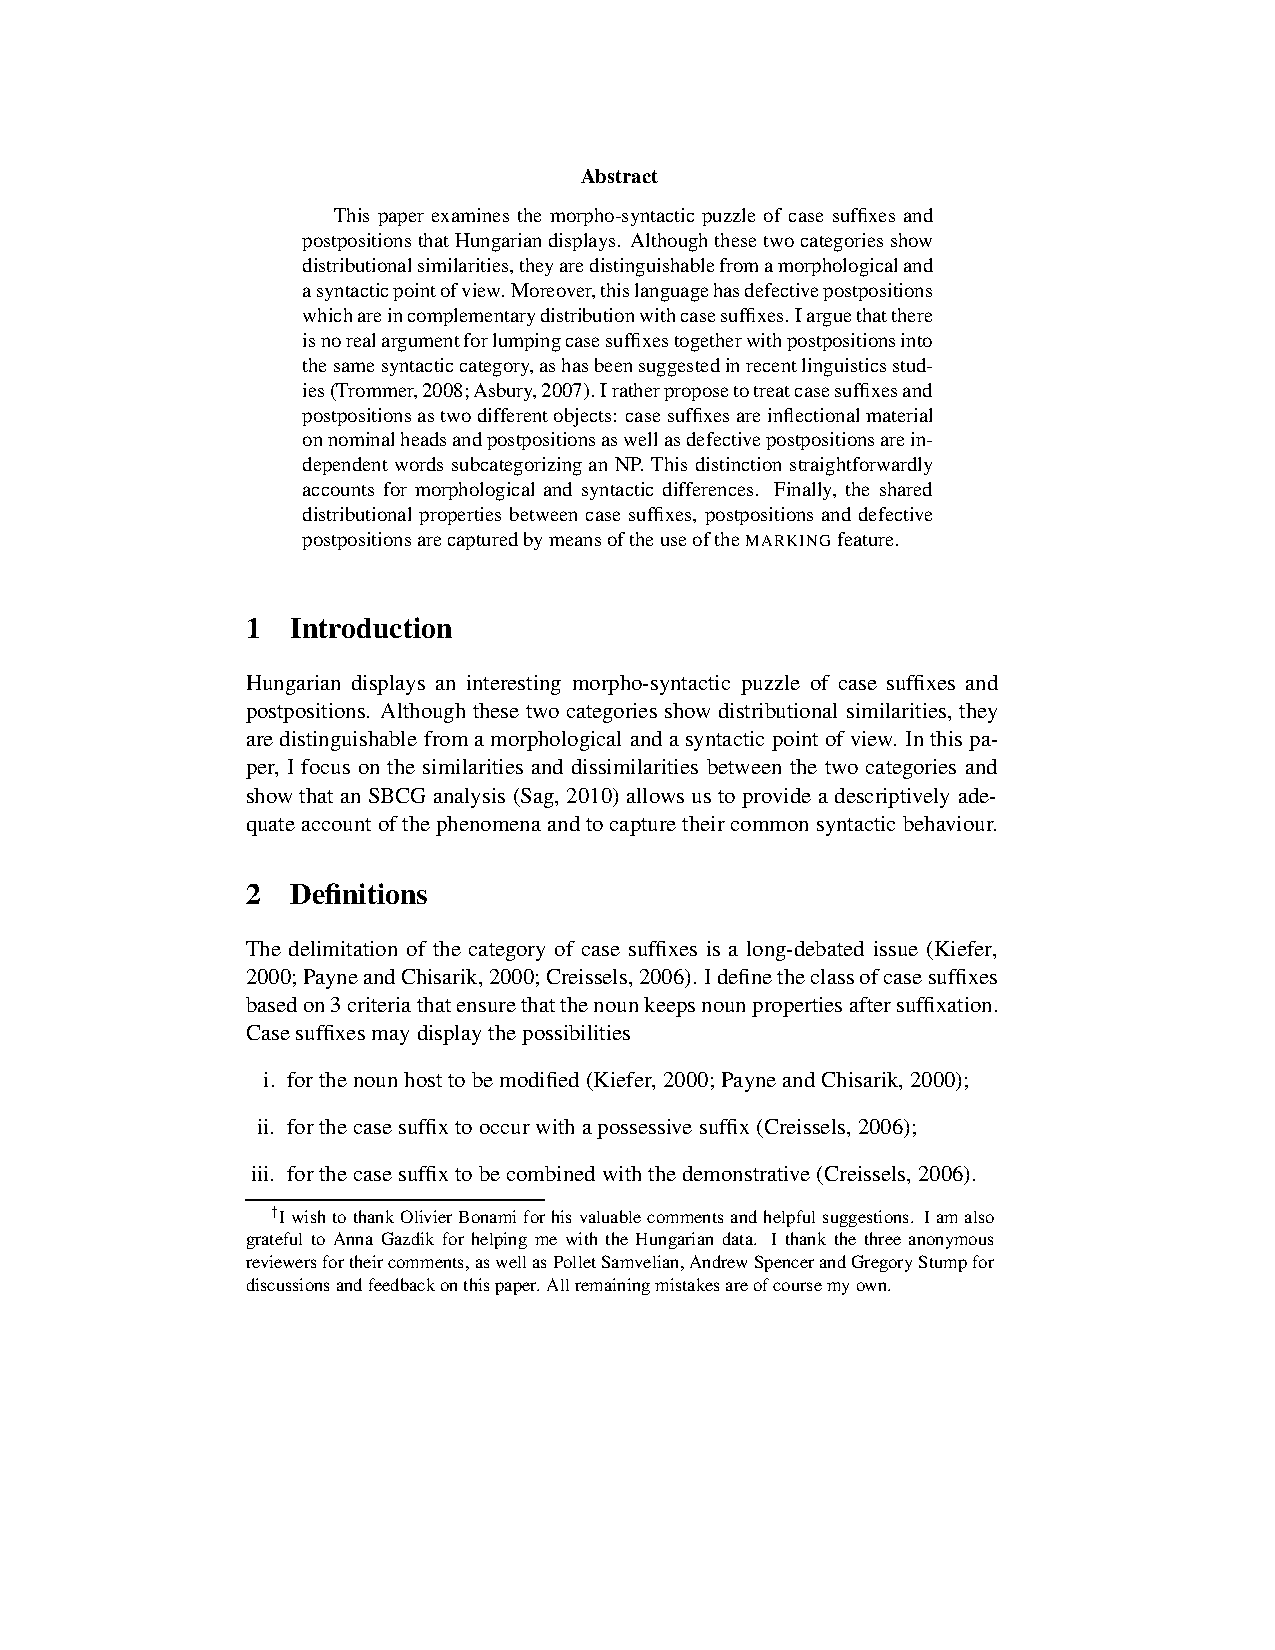
\includepdf[pages=-,pagecommand=\thispagestyle{plain}]{Includes/thuilier.pdf}
        \setcounter{page}{227}
        \phantomsection
        \addcontentsline{toc}{section}{Heike Walker: Adjuncts and the HPSG Binding Theory}
\thispagestyle{empty}

\begin{center}
  {\huge\bfseries Adjuncts and the HPSG Binding Theory\par}

  \bigskip

~\\
\begingroup
\setlength{\leftskip}{0pt plus 1fill}
\setlength{\rightskip}{0pt plus 1fill}
\setlength{\parindent}{0pt}
\setlength{\parfillskip}{0pt}
  \formatauthor{Heike Walker}{\begin{tabular}{@{}c@{}}University of Frankfurt am Main\end{tabular}}

\par\endgroup

  \vspace*{8ex}

  Proceedings of the 18th International Conference on\par Head-Driven Phrase Structure Grammar

  \bigskip

  University of Washington

  \medskip

  Stefan Müller (Editor)

  \medskip

  2011

  \medskip

  CSLI Publications

  \medskip

  pages 227--247

  \medskip

  \url{http://csli-publications.stanford.edu/HPSG/2011}
\end{center}
\vfill

\noindent



\vfill
\noindent
% APA Style
Walker, Heike. 2011. Adjuncts and the HPSG Binding Theory. In Müller, Stefan (Ed.), \emph{{Proceedings of the 18th International Conference on Head-Driven Phrase Structure Grammar, University of Washington}}, 227--247. Stanford,
CA: CSLI Publications. \hfill\href{http://creativecommons.org/licenses/by/4.0/}{\includegraphics[height=.75em]{Includes/ccby.eps}}

\newpage
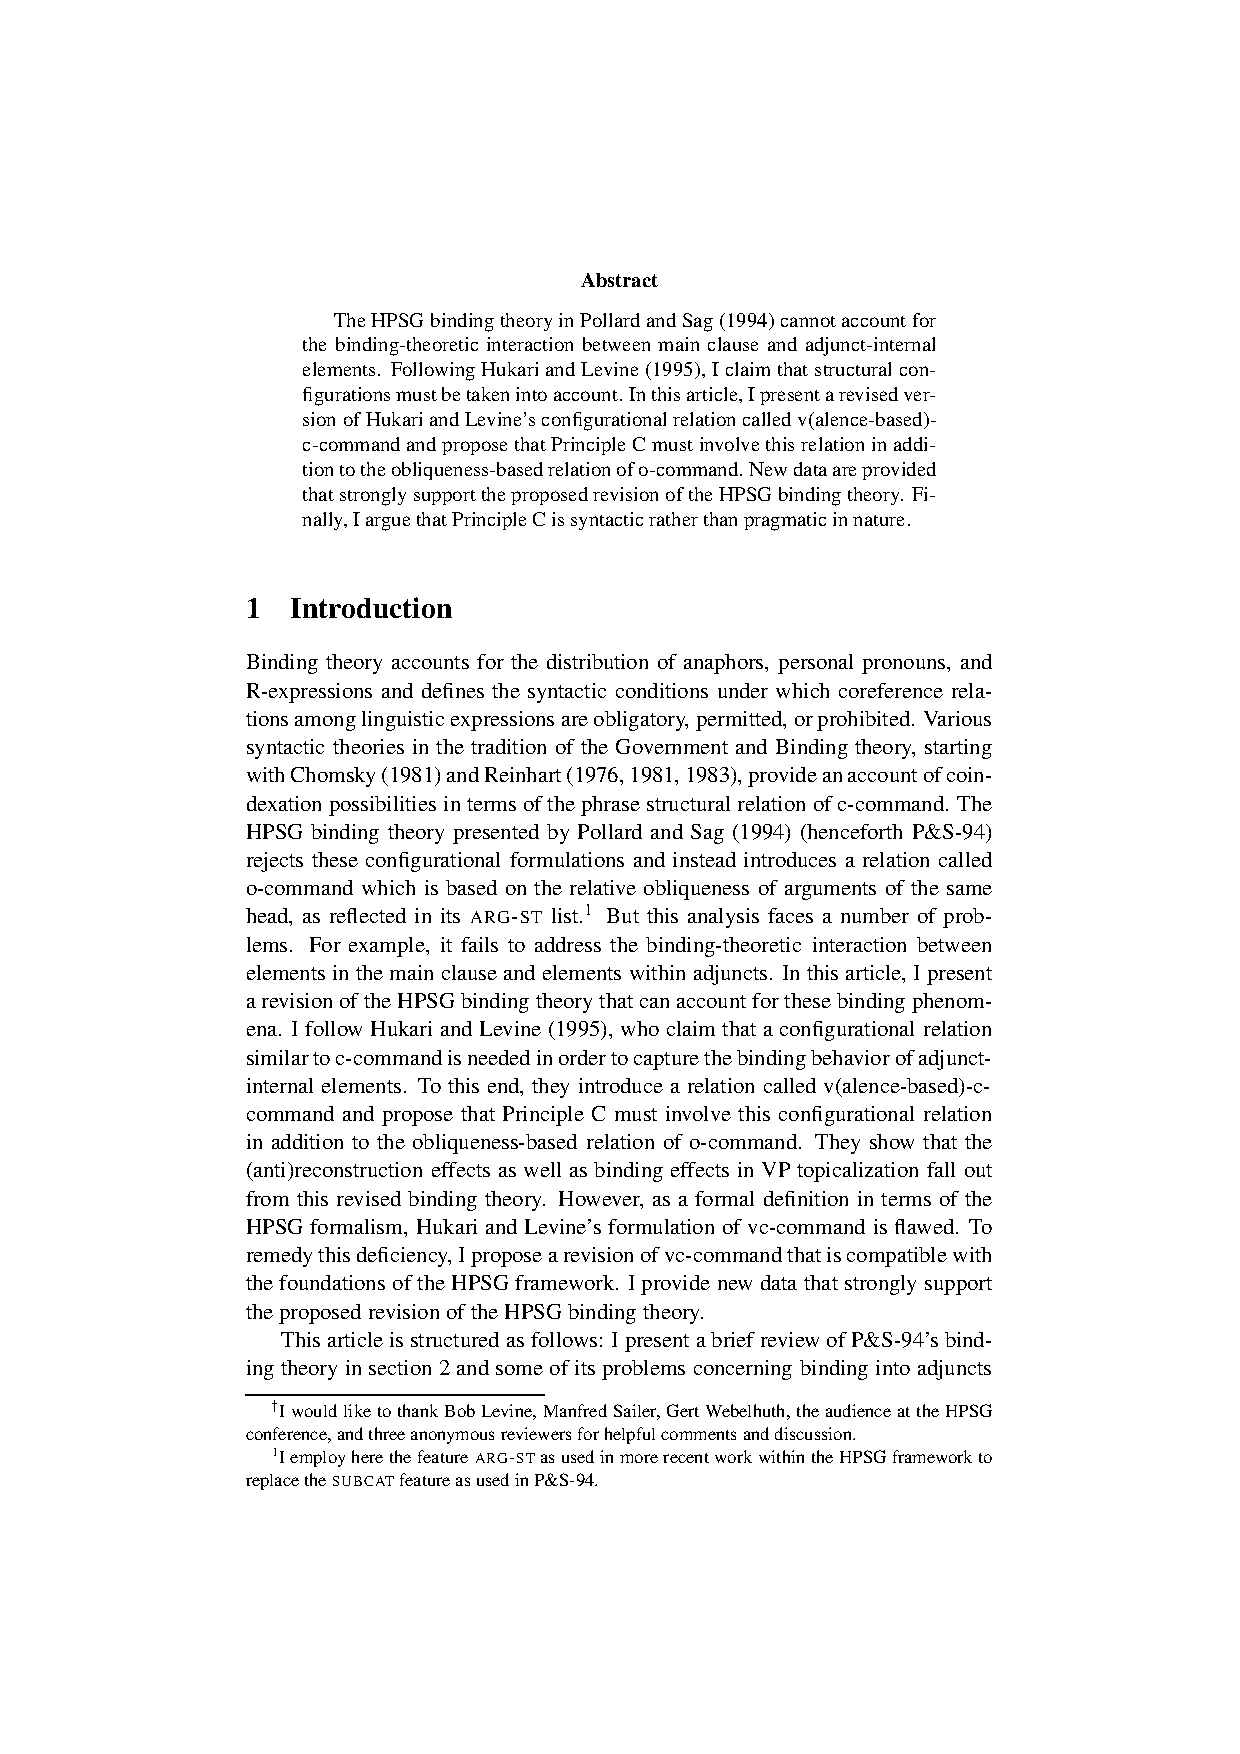
\includepdf[pages=-,pagecommand=\thispagestyle{plain}]{Includes/walker.pdf}
        \setcounter{page}{248}
        \phantomsection
        \addcontentsline{toc}{section}{Andrew C. Wetta: A Construction-based Cross-linguistic Analysis of V2 Word Order}
\thispagestyle{empty}

\begin{center}
  {\huge\bfseries A Construction-based Cross-linguistic Analysis of V2 Word Order\par}

  \bigskip

~\\
\begingroup
\setlength{\leftskip}{0pt plus 1fill}
\setlength{\rightskip}{0pt plus 1fill}
\setlength{\parindent}{0pt}
\setlength{\parfillskip}{0pt}
  \formatauthor{Andrew C. Wetta}{\begin{tabular}{@{}c@{}}University at Buffalo\end{tabular}}

\par\endgroup

  \vspace*{8ex}

  Proceedings of the 18th International Conference on\par Head-Driven Phrase Structure Grammar

  \bigskip

  University of Washington

  \medskip

  Stefan Müller (Editor)

  \medskip

  2011

  \medskip

  CSLI Publications

  \medskip

  pages 248--268

  \medskip

  \url{http://csli-publications.stanford.edu/HPSG/2011}
\end{center}
\vfill

\noindent



\vfill
\noindent
% APA Style
Wetta, Andrew C. 2011. A Construction-based Cross-linguistic Analysis of V2 Word Order. In Müller, Stefan (Ed.), \emph{{Proceedings of the 18th International Conference on Head-Driven Phrase Structure Grammar, University of Washington}}, 248--268. Stanford,
CA: CSLI Publications. \hfill\href{http://creativecommons.org/licenses/by/4.0/}{\includegraphics[height=.75em]{Includes/ccby.eps}}

\newpage
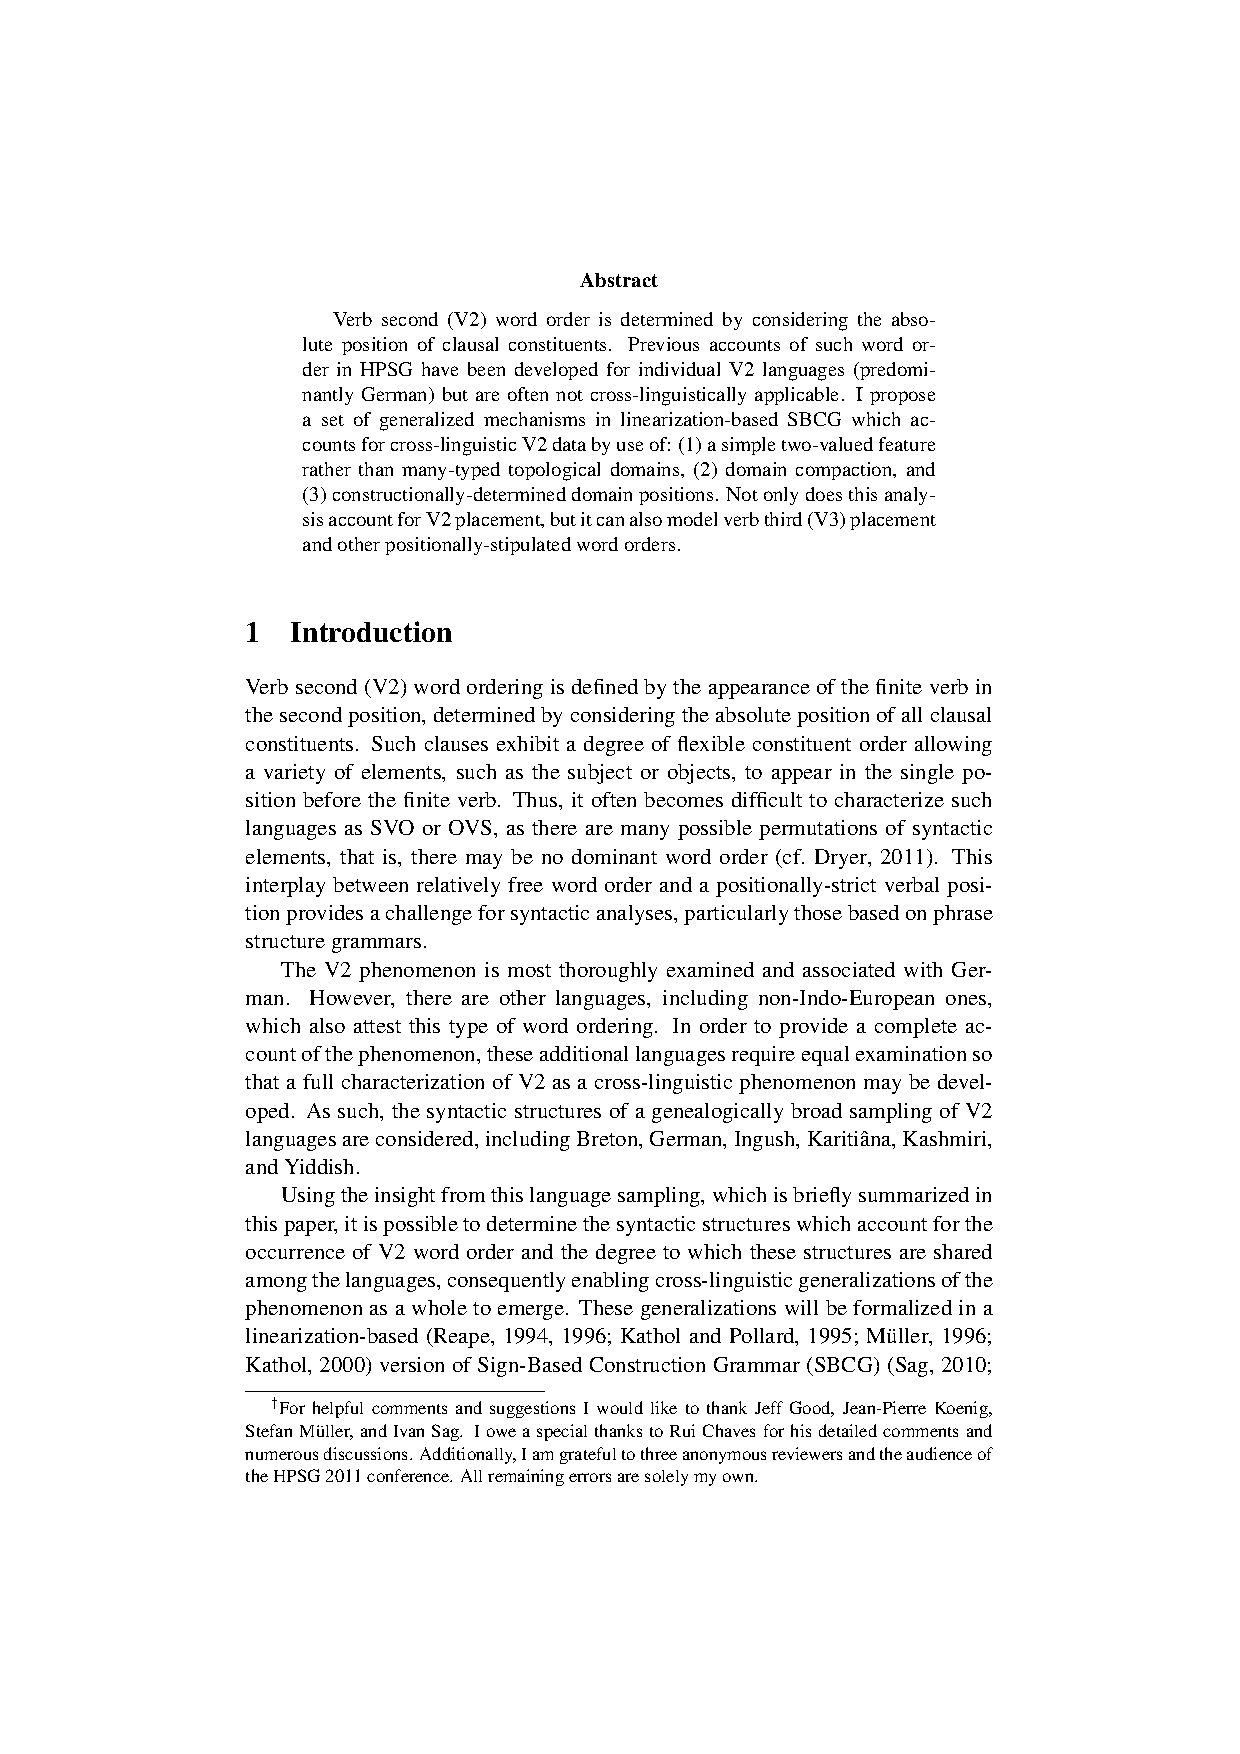
\includepdf[pages=-,pagecommand=\thispagestyle{plain}]{Includes/wetta.pdf}
\part{Contributions to the Workshop}
\thispagestyle{empty}
\newpage
        \setcounter{page}{270}
        \phantomsection
        \addcontentsline{toc}{section}{Anne Bjerre: Topic and focus in local subject extractions in Danish}
\thispagestyle{empty}

\begin{center}
  {\huge\bfseries Topic and focus in local subject extractions in Danish\par}

  \bigskip

~\\
\begingroup
\setlength{\leftskip}{0pt plus 1fill}
\setlength{\rightskip}{0pt plus 1fill}
\setlength{\parindent}{0pt}
\setlength{\parfillskip}{0pt}
  \formatauthor{Anne Bjerre}{\begin{tabular}{@{}c@{}}University of Southern Denmark\end{tabular}}

\par\endgroup

  \vspace*{8ex}

  Proceedings of the 18th International Conference on\par Head-Driven Phrase Structure Grammar

  \bigskip

  University of Washington

  \medskip

  Stefan Müller (Editor)

  \medskip

  2011

  \medskip

  CSLI Publications

  \medskip

  pages 270--288

  \medskip

  \url{http://csli-publications.stanford.edu/HPSG/2011}
\end{center}
\vfill

\noindent



\vfill
\noindent
% APA Style
Bjerre, Anne. 2011. Topic and focus in local subject extractions in Danish. In Müller, Stefan (Ed.), \emph{{Proceedings of the 18th International Conference on Head-Driven Phrase Structure Grammar, University of Washington}}, 270--288. Stanford,
CA: CSLI Publications. \hfill\href{http://creativecommons.org/licenses/by/4.0/}{\includegraphics[height=.75em]{Includes/ccby.eps}}

\newpage
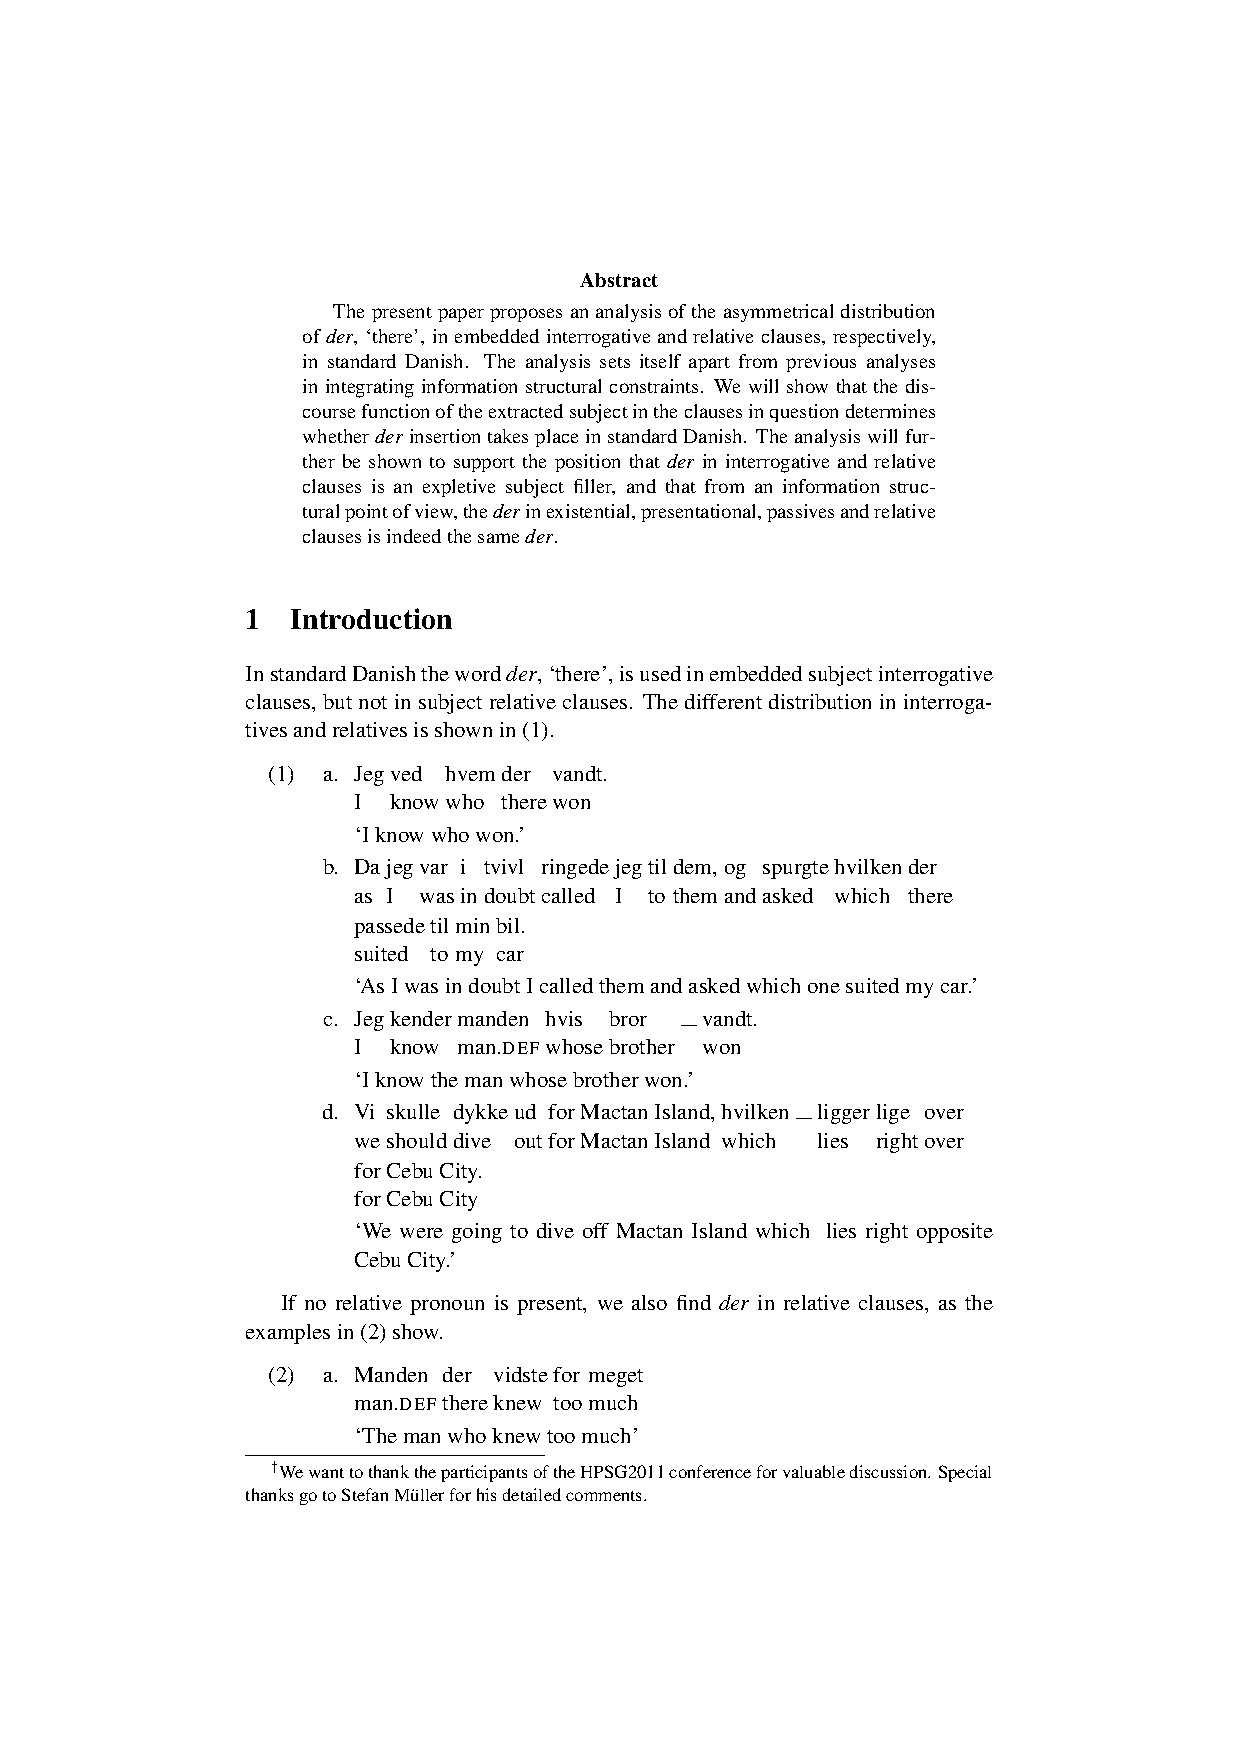
\includepdf[pages=-,pagecommand=\thispagestyle{plain}]{Includes/bjerre.pdf}
        \setcounter{page}{289}
        \phantomsection
        \addcontentsline{toc}{section}{Kordula De Kuthy, Detmar Meurers: Integrating GIVENness into a structured meaning approach in HPSG}
\thispagestyle{empty}

\begin{center}
  {\huge\bfseries Integrating GIVENness into a structured meaning approach in HPSG\par}

  \bigskip

~\\
\begingroup
\setlength{\leftskip}{0pt plus 1fill}
\setlength{\rightskip}{0pt plus 1fill}
\setlength{\parindent}{0pt}
\setlength{\parfillskip}{0pt}
  \formatauthor{Kordula De Kuthy}{\begin{tabular}{@{}c@{}}Universität Tübingen\end{tabular}}
\formatauthor{Detmar Meurers}{\begin{tabular}{@{}c@{}}Universität Tübingen\end{tabular}}

\par\endgroup

  \vspace*{8ex}

  Proceedings of the 18th International Conference on\par Head-Driven Phrase Structure Grammar

  \bigskip

  University of Washington

  \medskip

  Stefan Müller (Editor)

  \medskip

  2011

  \medskip

  CSLI Publications

  \medskip

  pages 289--301

  \medskip

  \url{http://csli-publications.stanford.edu/HPSG/2011}
\end{center}
\vfill

\noindent



\vfill
\noindent
% APA Style
De Kuthy, Kordula, \& Meurers, Detmar. 2011. Integrating GIVENness into a structured meaning approach in HPSG. In Müller, Stefan (Ed.), \emph{{Proceedings of the 18th International Conference on Head-Driven Phrase Structure Grammar, University of Washington}}, 289--301. Stanford,
CA: CSLI Publications. \hfill\href{http://creativecommons.org/licenses/by/4.0/}{\includegraphics[height=.75em]{Includes/ccby.eps}}

\newpage
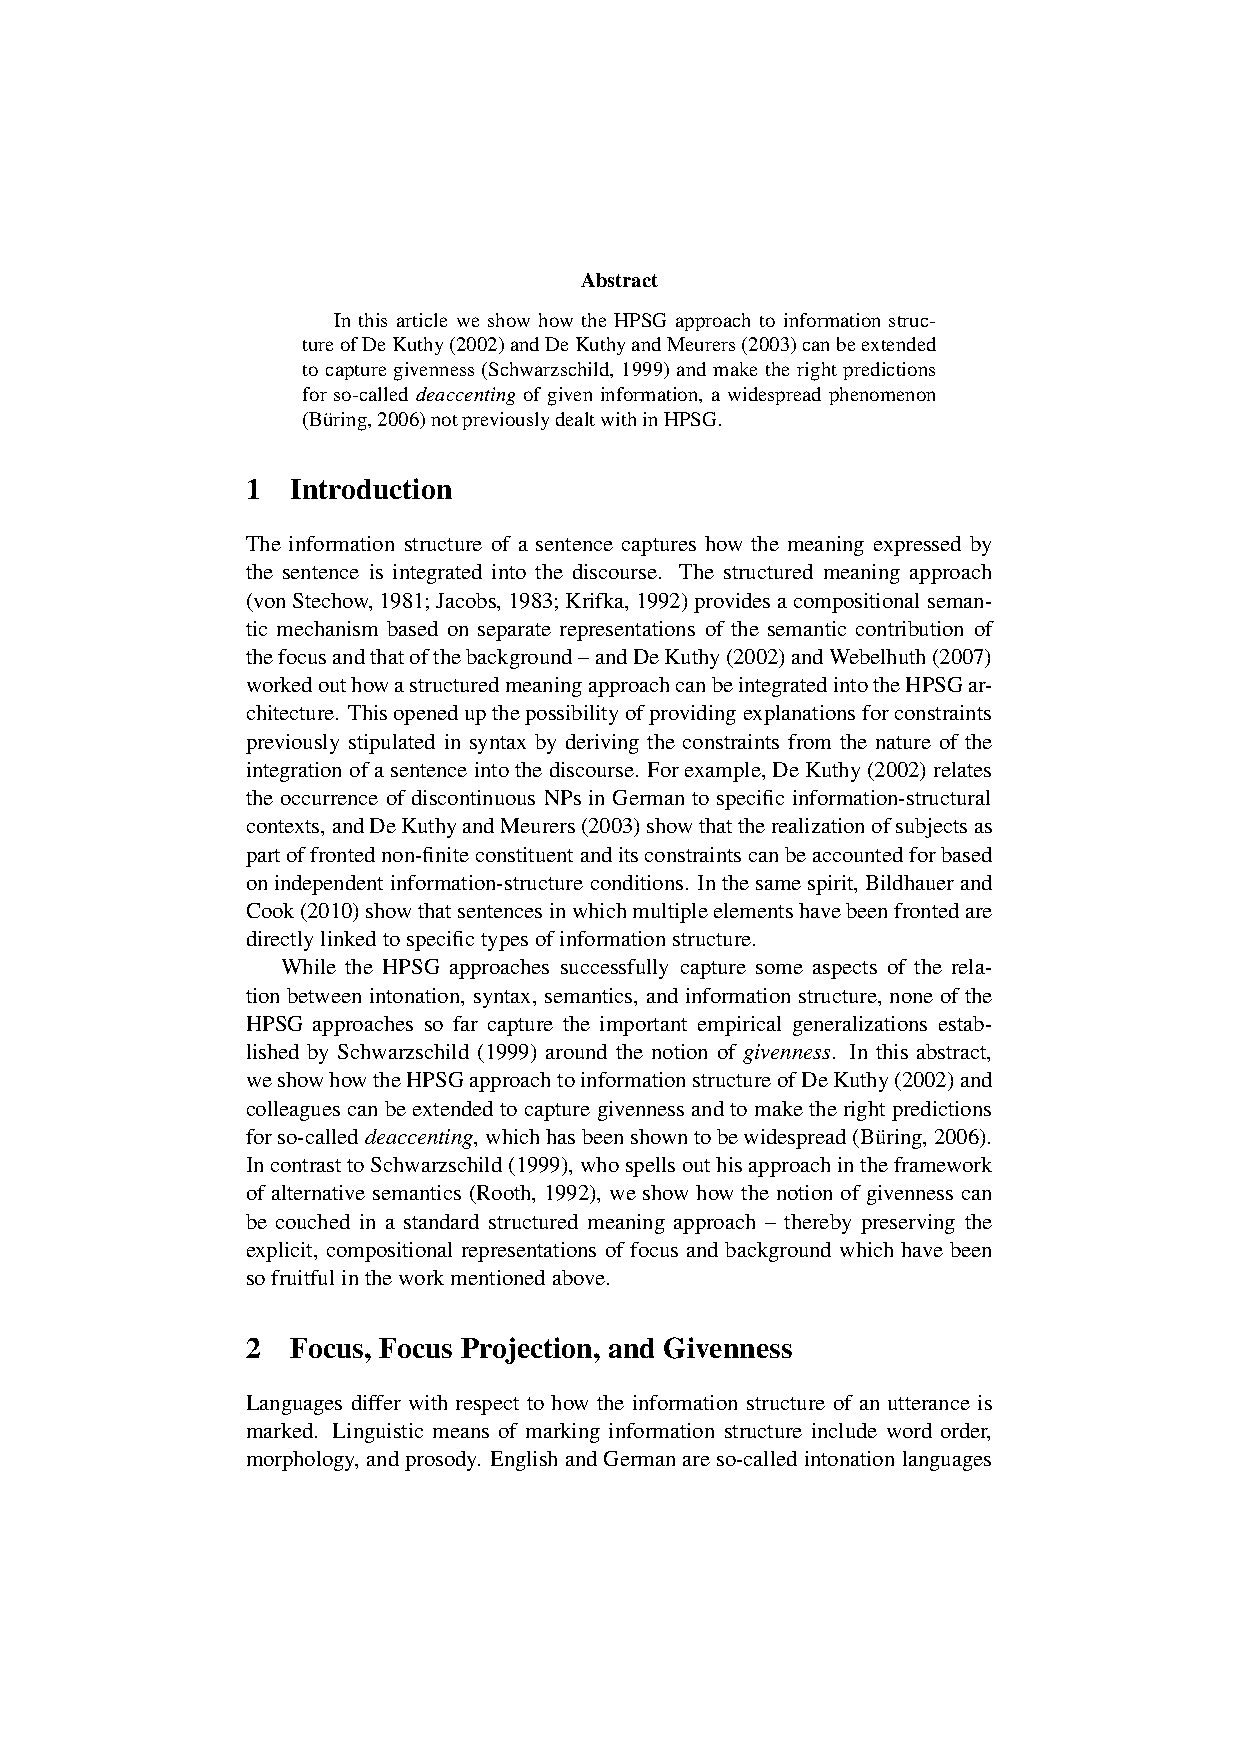
\includepdf[pages=-,pagecommand=\thispagestyle{plain}]{Includes/dekuthy-meurers.pdf}
        \setcounter{page}{302}
        \phantomsection
        \addcontentsline{toc}{section}{Jong-Bok Kim: Floating Numeral Classifiers in Korean: A Thematic-Structure Perspective}
\thispagestyle{empty}

\begin{center}
  {\huge\bfseries Floating Numeral Classifiers in Korean: A Thematic-Structure Perspective\par}

  \bigskip

~\\
\begingroup
\setlength{\leftskip}{0pt plus 1fill}
\setlength{\rightskip}{0pt plus 1fill}
\setlength{\parindent}{0pt}
\setlength{\parfillskip}{0pt}
  \formatauthor{Jong-Bok Kim}{\begin{tabular}{@{}c@{}}Kyung Hee University\end{tabular}}

\par\endgroup

  \vspace*{8ex}

  Proceedings of the 18th International Conference on\par Head-Driven Phrase Structure Grammar

  \bigskip

  University of Washington

  \medskip

  Stefan Müller (Editor)

  \medskip

  2011

  \medskip

  CSLI Publications

  \medskip

  pages 302--313

  \medskip

  \url{http://csli-publications.stanford.edu/HPSG/2011}
\end{center}
\vfill

\noindent



\vfill
\noindent
% APA Style
Kim, Jong-Bok. 2011. Floating Numeral Classifiers in Korean: A Thematic-Structure Perspective. In Müller, Stefan (Ed.), \emph{{Proceedings of the 18th International Conference on Head-Driven Phrase Structure Grammar, University of Washington}}, 302--313. Stanford,
CA: CSLI Publications. \hfill\href{http://creativecommons.org/licenses/by/4.0/}{\includegraphics[height=.75em]{Includes/ccby.eps}}

\newpage
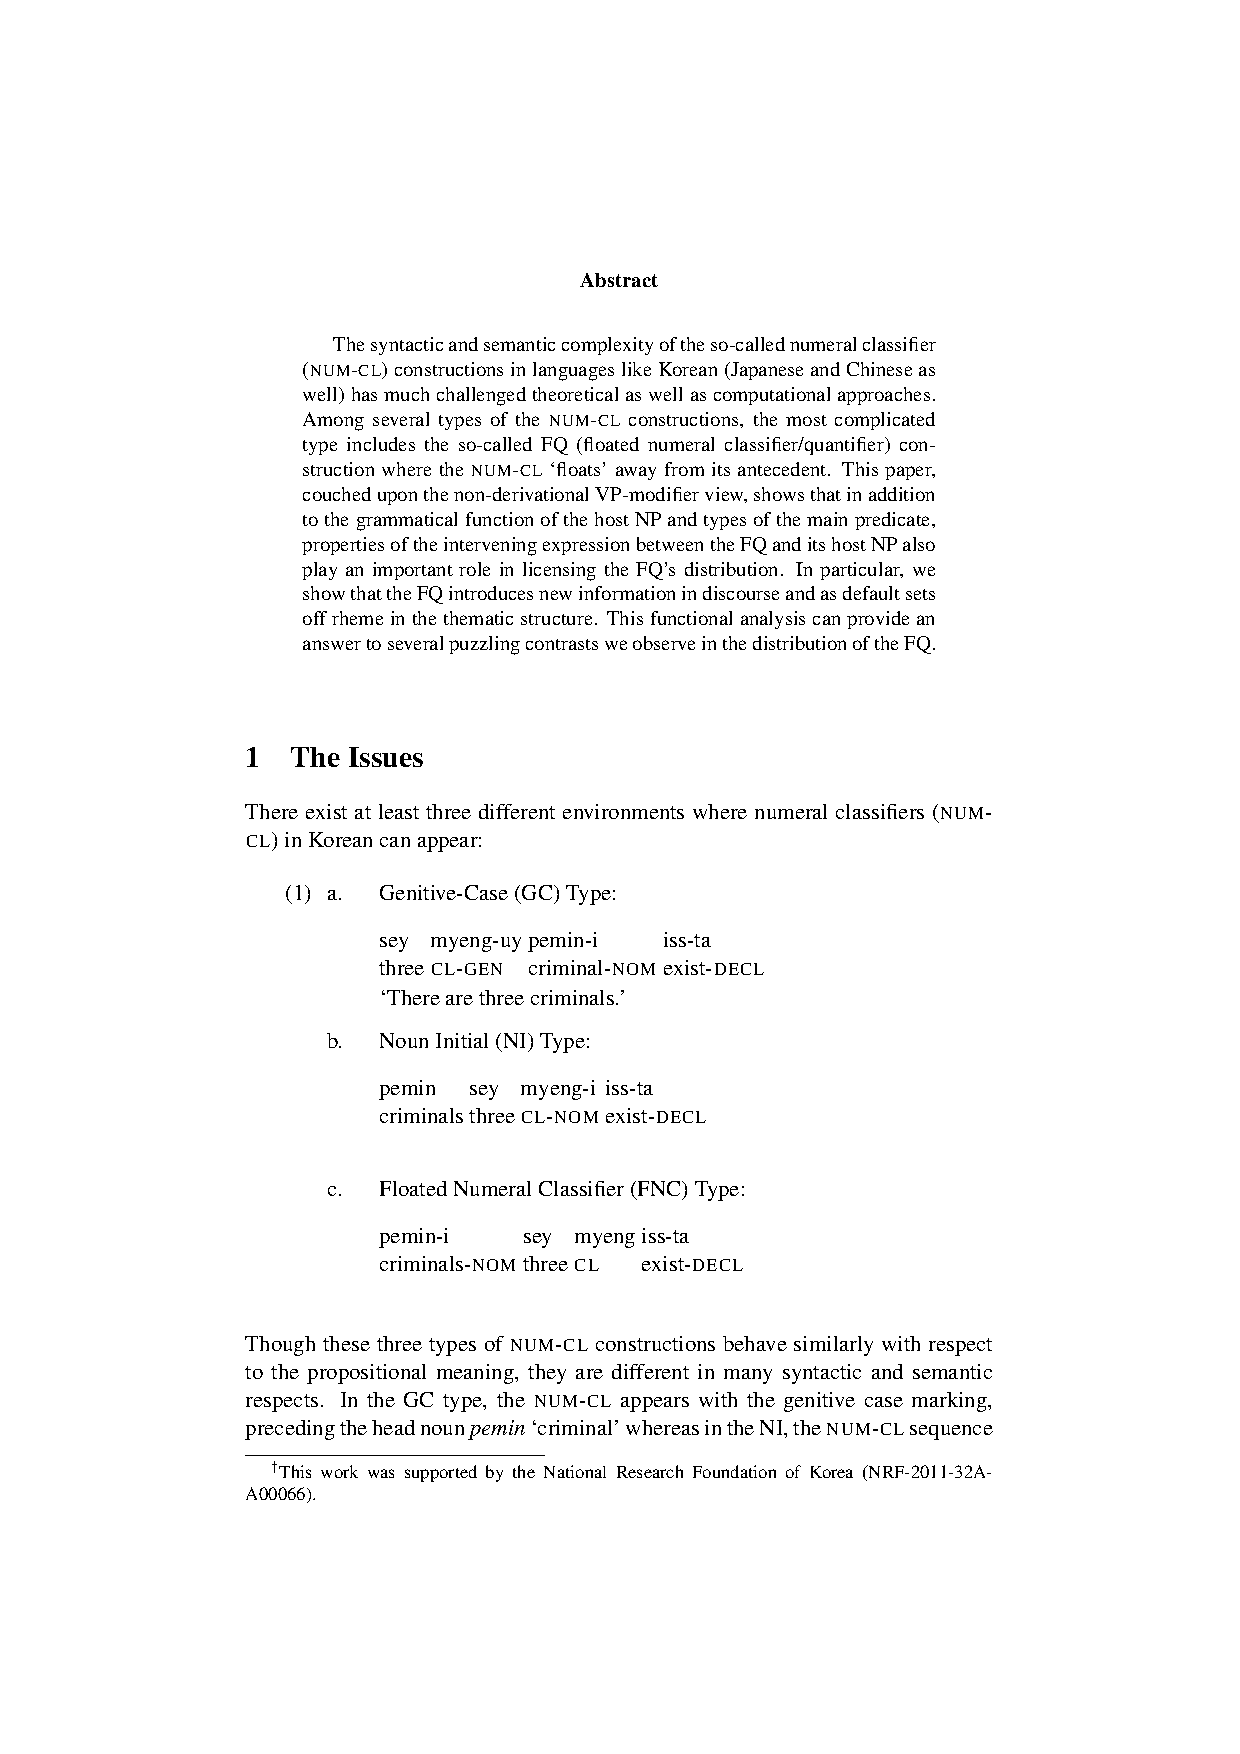
\includepdf[pages=-,pagecommand=\thispagestyle{plain}]{Includes/kim.pdf}
        \setcounter{page}{314}
        \phantomsection
        \addcontentsline{toc}{section}{Caitlin Light: The information structure of subject extraposition in Early New High German}
\thispagestyle{empty}

\begin{center}
  {\huge\bfseries The information structure of subject extraposition in Early New High German\par}

  \bigskip

~\\
\begingroup
\setlength{\leftskip}{0pt plus 1fill}
\setlength{\rightskip}{0pt plus 1fill}
\setlength{\parindent}{0pt}
\setlength{\parfillskip}{0pt}
  \formatauthor{Caitlin Light}{\begin{tabular}{@{}c@{}}University of Pennsylvania\end{tabular}}

\par\endgroup

  \vspace*{8ex}

  Proceedings of the 18th International Conference on\par Head-Driven Phrase Structure Grammar

  \bigskip

  University of Washington

  \medskip

  Stefan Müller (Editor)

  \medskip

  2011

  \medskip

  CSLI Publications

  \medskip

  pages 314--326

  \medskip

  \url{http://csli-publications.stanford.edu/HPSG/2011}
\end{center}
\vfill

\noindent



\vfill
\noindent
% APA Style
Light, Caitlin. 2011. The information structure of subject extraposition in Early New High German. In Müller, Stefan (Ed.), \emph{{Proceedings of the 18th International Conference on Head-Driven Phrase Structure Grammar, University of Washington}}, 314--326. Stanford,
CA: CSLI Publications. \hfill\href{http://creativecommons.org/licenses/by/4.0/}{\includegraphics[height=.75em]{Includes/ccby.eps}}

\newpage
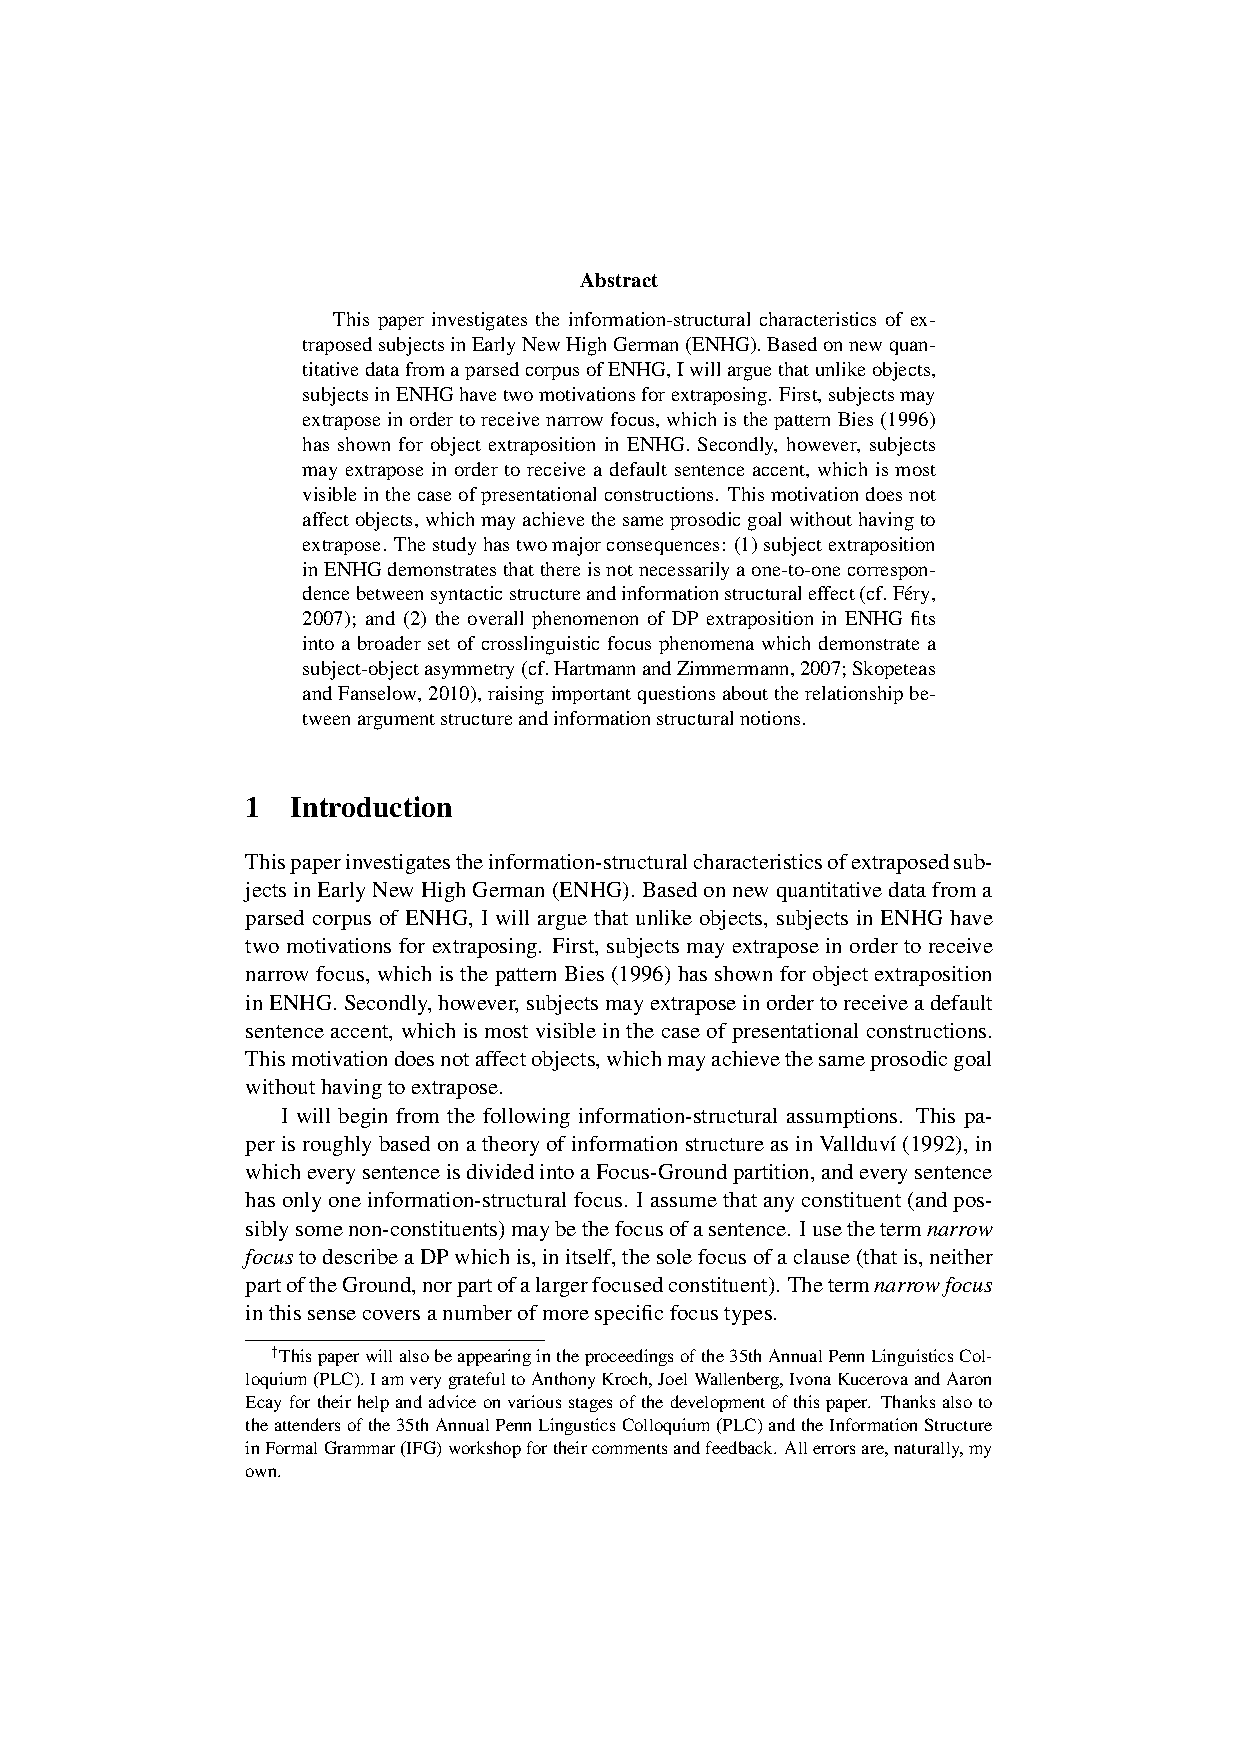
\includepdf[pages=-,pagecommand=\thispagestyle{plain}]{Includes/light.pdf}
        \setcounter{page}{327}
        \phantomsection
        \addcontentsline{toc}{section}{Jean-Marie Marandin: Subject Inversion in French. The Limits of Information Structure}
\thispagestyle{empty}

\begin{center}
  {\huge\bfseries Subject Inversion in French. The Limits of Information Structure\par}

  \bigskip

~\\
\begingroup
\setlength{\leftskip}{0pt plus 1fill}
\setlength{\rightskip}{0pt plus 1fill}
\setlength{\parindent}{0pt}
\setlength{\parfillskip}{0pt}
  \formatauthor{Jean-Marie Marandin}{\begin{tabular}{@{}c@{}}CNRS, Université Paris Diderot\end{tabular}}

\par\endgroup

  \vspace*{8ex}

  Proceedings of the 18th International Conference on\par Head-Driven Phrase Structure Grammar

  \bigskip

  University of Washington

  \medskip

  Stefan Müller (Editor)

  \medskip

  2011

  \medskip

  CSLI Publications

  \medskip

  pages 327--347

  \medskip

  \url{http://csli-publications.stanford.edu/HPSG/2011}
\end{center}
\vfill

\noindent



\vfill
\noindent
% APA Style
Marandin, Jean-Marie. 2011. Subject Inversion in French. The Limits of Information Structure. In Müller, Stefan (Ed.), \emph{{Proceedings of the 18th International Conference on Head-Driven Phrase Structure Grammar, University of Washington}}, 327--347. Stanford,
CA: CSLI Publications. \hfill\href{http://creativecommons.org/licenses/by/4.0/}{\includegraphics[height=.75em]{Includes/ccby.eps}}

\newpage
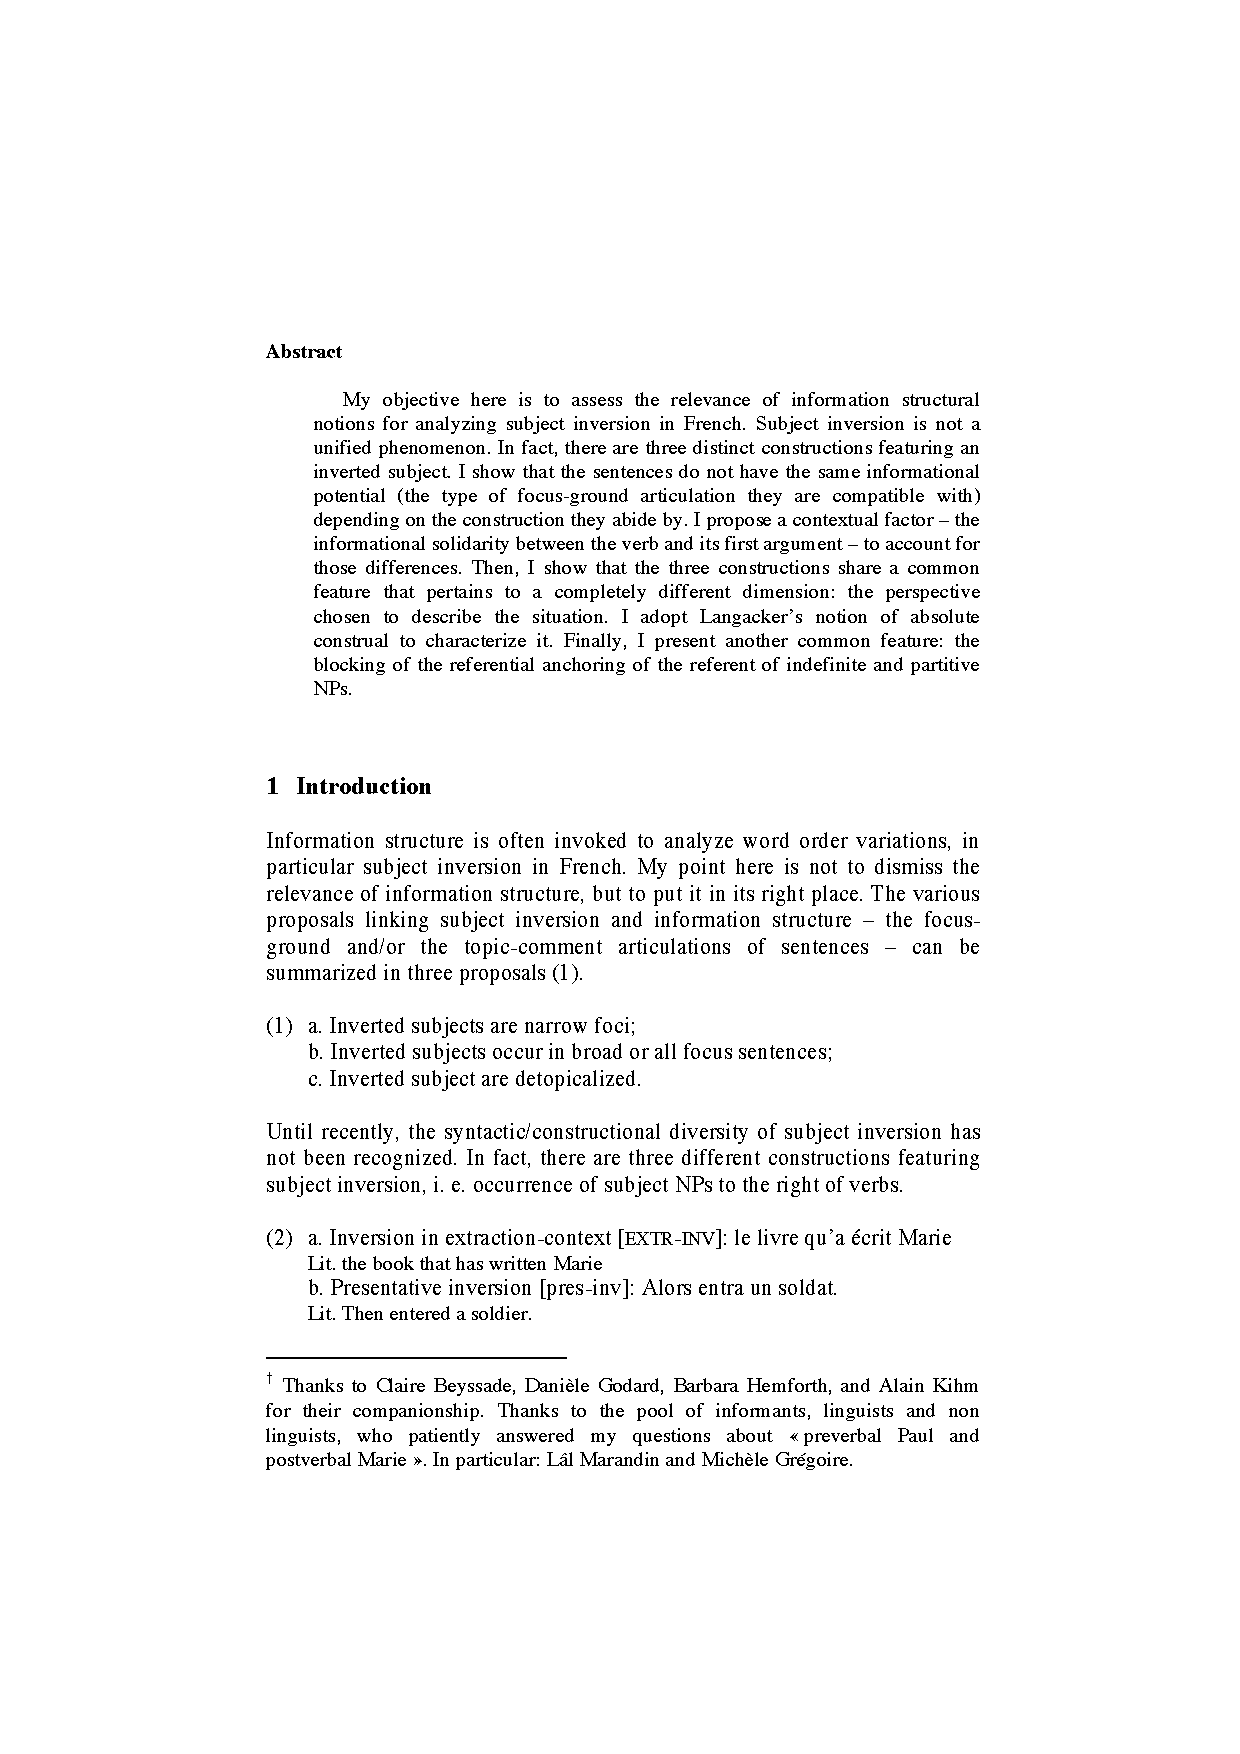
\includepdf[pages=-,pagecommand=\thispagestyle{plain}]{Includes/marandin.pdf}
        \setcounter{page}{348}
        \phantomsection
        \addcontentsline{toc}{section}{Sanghoun Song, Emily M. Bender: Using Information Structure to Improve Transfer-based MT}
\thispagestyle{empty}

\begin{center}
  {\huge\bfseries Using Information Structure to Improve Transfer-based MT\par}

  \bigskip

~\\
\begingroup
\setlength{\leftskip}{0pt plus 1fill}
\setlength{\rightskip}{0pt plus 1fill}
\setlength{\parindent}{0pt}
\setlength{\parfillskip}{0pt}
  \formatauthor{Sanghoun Song}{\begin{tabular}{@{}c@{}}University of Washington\end{tabular}}
\formatauthor{Emily M. Bender}{\begin{tabular}{@{}c@{}}University of Washington\end{tabular}}

\par\endgroup

  \vspace*{8ex}

  Proceedings of the 18th International Conference on\par Head-Driven Phrase Structure Grammar

  \bigskip

  University of Washington

  \medskip

  Stefan Müller (Editor)

  \medskip

  2011

  \medskip

  CSLI Publications

  \medskip

  pages 348--368

  \medskip

  \url{http://csli-publications.stanford.edu/HPSG/2011}
\end{center}
\vfill

\noindent



\vfill
\noindent
% APA Style
Song, Sanghoun, \& Bender, Emily M. 2011. Using Information Structure to Improve Transfer-based MT. In Müller, Stefan (Ed.), \emph{{Proceedings of the 18th International Conference on Head-Driven Phrase Structure Grammar, University of Washington}}, 348--368. Stanford,
CA: CSLI Publications. \hfill\href{http://creativecommons.org/licenses/by/4.0/}{\includegraphics[height=.75em]{Includes/ccby.eps}}

\newpage
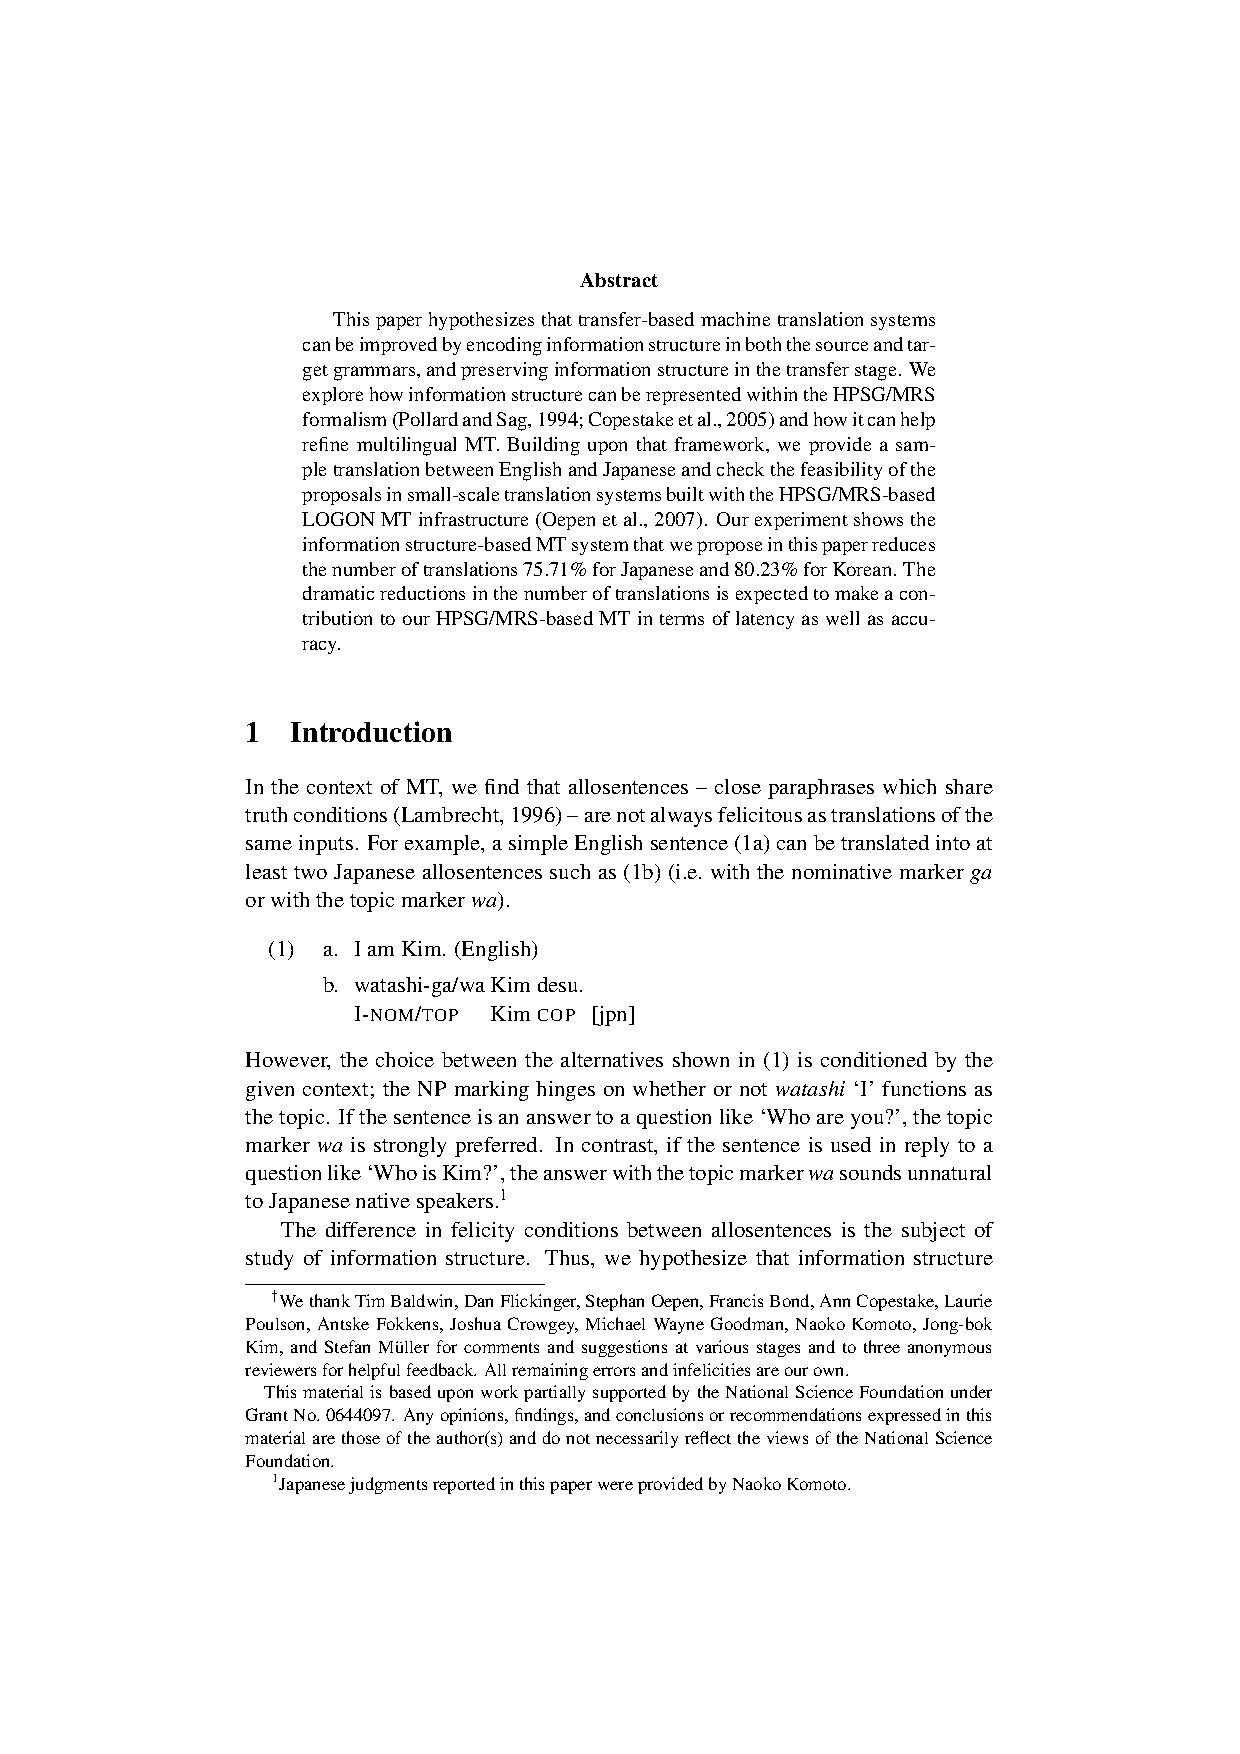
\includepdf[pages=-,pagecommand=\thispagestyle{plain}]{Includes/song-bender.pdf}
        \setcounter{page}{369}
        \phantomsection
        \addcontentsline{toc}{section}{Jon Stevens: Information Structure as Parallel Tree Building}
\thispagestyle{empty}

\begin{center}
  {\huge\bfseries Information Structure as Parallel Tree Building\par}

  \bigskip

~\\
\begingroup
\setlength{\leftskip}{0pt plus 1fill}
\setlength{\rightskip}{0pt plus 1fill}
\setlength{\parindent}{0pt}
\setlength{\parfillskip}{0pt}
  \formatauthor{Jon Stevens}{\begin{tabular}{@{}c@{}}University of Pennsylvania\end{tabular}}

\par\endgroup

  \vspace*{8ex}

  Proceedings of the 18th International Conference on\par Head-Driven Phrase Structure Grammar

  \bigskip

  University of Washington

  \medskip

  Stefan Müller (Editor)

  \medskip

  2011

  \medskip

  CSLI Publications

  \medskip

  pages 369--386

  \medskip

  \url{http://csli-publications.stanford.edu/HPSG/2011}
\end{center}
\vfill

\noindent



\vfill
\noindent
% APA Style
Stevens, Jon. 2011. Information Structure as Parallel Tree Building. In Müller, Stefan (Ed.), \emph{{Proceedings of the 18th International Conference on Head-Driven Phrase Structure Grammar, University of Washington}}, 369--386. Stanford,
CA: CSLI Publications. \hfill\href{http://creativecommons.org/licenses/by/4.0/}{\includegraphics[height=.75em]{Includes/ccby.eps}}

\newpage
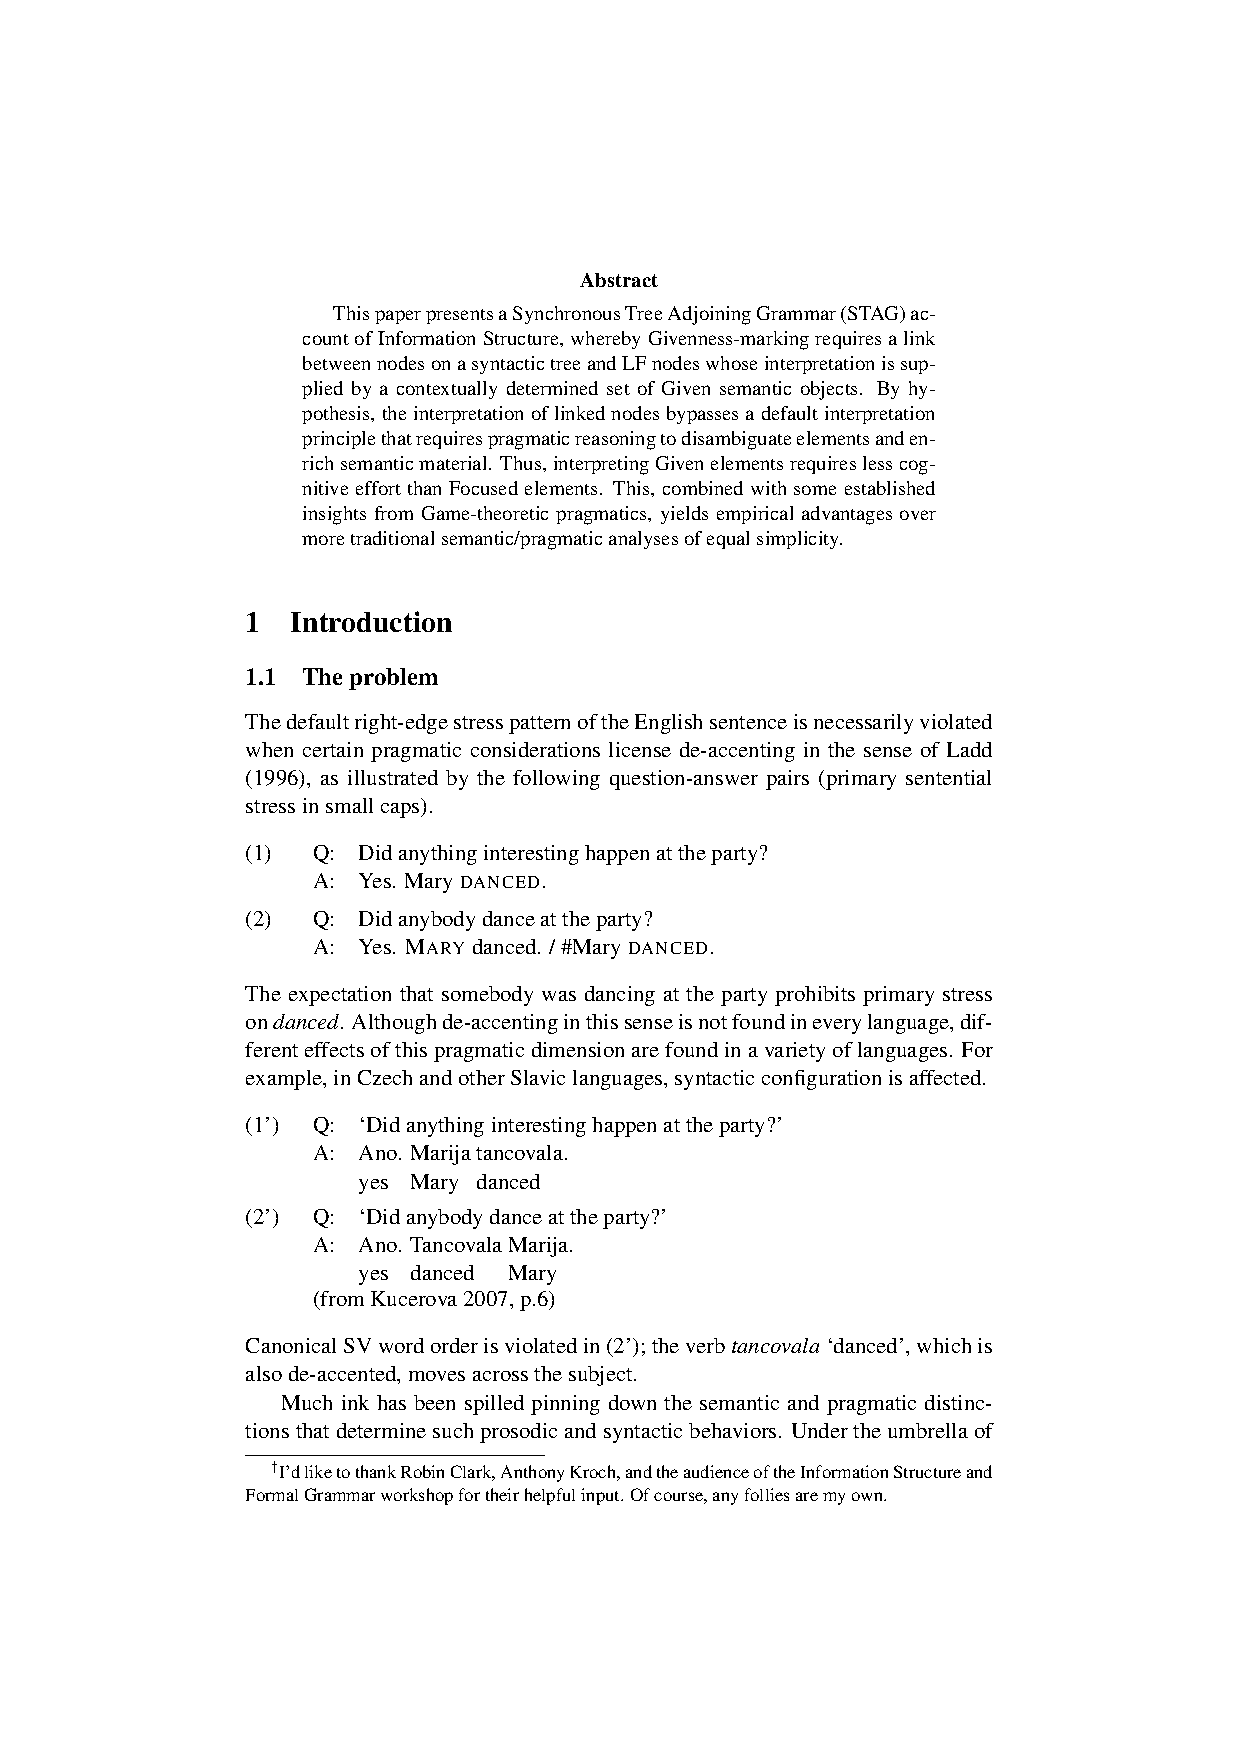
\includepdf[pages=-,pagecommand=\thispagestyle{plain}]{Includes/stevens.pdf}
\end{document}
